% =====================================================================
% گزارش فنی فارسی - فصل چهارم: کنترل مقاوم و تطبیقی L1
% کامپایل با: latexmk -xelatex ch4_report_fa.tex
% (xelatex -> biber -> xelatex -> xelatex)
%
% همه اعداد این گزارش از پیاده‌سازی Chapter4/ اندازه‌گیری شده‌اند؛ منبع هر
% عدد در docs/CH4_UNCERTAINTY.md بخش 5a و در نسخه انگلیسی ch4_report.html آمده است.
% =====================================================================
\documentclass[10pt,twocolumn]{article}

% ---------------------- بسته‌های پایه ----------------------
\usepackage{geometry}
\geometry{a4paper, top=2cm, bottom=2.2cm, left=1.8cm, right=1.8cm, columnsep=0.7cm}

\usepackage{array}

\usepackage{xepersian}

% ---------------------- انتخاب فونت (با بازگشت خودکار) ----------------------
% فونت متن اصلی: B Nazanin. این فونت فاقد نویسه‌های «٪» و «٫» است،
% بنابراین فونت اعداد را از فونت دیگری با پوشش کامل یونیکد تأمین می‌کنیم.
\IfFontExistsTF{B Nazanin}
    {\settextfont{B Nazanin}}
    {\IfFontExistsTF{XB Niloofar}
        {\settextfont{XB Niloofar}}
        {\settextfont{Vazirmatn}}}

\IfFontExistsTF{Geeza Pro}
    {\setdigitfont{Geeza Pro}}
    {\IfFontExistsTF{Damascus}
        {\setdigitfont{Damascus}}
        {\IfFontExistsTF{Vazirmatn}
            {\setdigitfont{Vazirmatn}}
            {\setdigitfont{B Nazanin}}}}

\IfFontExistsTF{Times New Roman}
    {\setlatintextfont{Times New Roman}}
    {\setlatintextfont{FreeSerif}}

\usepackage{amsmath,amssymb}
\usepackage{graphicx}
\graphicspath{{figures/}}
\usepackage{caption}
\usepackage{booktabs}
\usepackage{float}
\usepackage[hidelinks]{hyperref}
\usepackage{fancyhdr}
\usepackage{titlesec}
\usepackage[backend=biber,style=ieee,sorting=none]{biblatex}
\addbibresource{references.bib}

% ---------------------- دستورهای کمکی ----------------------
% B Nazanin نویسه‌های خط تیره را ندارد؛ آن‌ها را از فونت لاتین می‌گیریم.
\newcommand{\en}[1]{\lr{#1}}
\newcommand{\code}[1]{\lr{\texttt{#1}}}
\newcommand{\md}{\lr{\textemdash}}
\newcommand{\nd}{\lr{\textendash}}
\newcommand{\Lone}{\texorpdfstring{$\mathcal{L}_1$}{L1}}
% خانه جدول نتایج: تعداد گام · بیشینه خطا · کمینه نیروی عمودی
\newcommand{\rc}[3]{${#1}\;|\;{#2}\;|\;{#3}$}
% steps | valid steps | max||eta|| | min Fz
\newcommand{\rcv}[4]{${#1}\;|\;{#2}\;|\;{#3}\;|\;{#4}$}
\newcommand{\fall}[1]{$\mathbf{#1}^{\dagger}$}
\newcommand{\fallc}[3]{$\mathbf{#1}^{\dagger}\;|\;{#2}\;|\;{#3}$}

% فهرست مراجع تماماً لاتین است و باید با فونت و جهت لاتین چیده شود.
\AtBeginBibliography{\setlatin}
\renewcommand*{\bibfont}{\latinfont\footnotesize}

% ---------------------- شناورها ----------------------
\renewcommand{\topfraction}{0.9}
\renewcommand{\bottomfraction}{0.8}
\renewcommand{\textfraction}{0.07}
\renewcommand{\floatpagefraction}{0.7}
\renewcommand{\dbltopfraction}{0.8}
\renewcommand{\dblfloatpagefraction}{0.7}
\setcounter{topnumber}{3}
\setcounter{dbltopnumber}{2}
\setcounter{totalnumber}{5}

% ---------------------- تنظیم عنوان بخش‌ها ----------------------
\titleformat{\section}{\normalfont\bfseries\large}{\thesection.}{0.5em}{}
\titleformat{\subsection}{\normalfont\bfseries}{\thesubsection.}{0.5em}{}

% ---------------------- سربرگ و پابرگ ----------------------
\pagestyle{fancy}
\fancyhf{}
\fancyhead[C]{گزارش فنی \nd{} \small کنترل مقاوم و تطبیقی $\mathcal{L}_1$ برای راه‌رفتن ربات دوپا}
\fancyfoot[C]{\thepage}
\renewcommand{\headrulewidth}{0.4pt}

% ---------------------- اطلاعات سند ----------------------
\newcommand{\reporttitle}{کنترل مقاوم و تطبیقی $\mathcal{L}_1$ برای راه‌رفتن ربات دوپا:\\[0.2em]
بازتولید و اعتبارسنجی عددی فصل چهارم}
\newcommand{\reportauthor}{محمد ملک}
\newcommand{\reportaffil}{پروژه ربات دوپای \en{RABBIT} \nd{} مدل‌سازی، کنترل و بهینه‌سازی مسیر}
\newcommand{\reportemail}{malek.mohammad132@gmail.com}

% =====================================================================
\begin{document}

\onecolumn
\begin{center}
    {\bfseries\Large \reporttitle}\\[0.8em]
    \reportauthor \\
    \small \reportaffil \\
    \small \texttt{\reportemail} \\[0.3em]
    \today
\end{center}
\vspace{1em}

\begin{center}
    {\bfseries\large چکیده}
\end{center}
\noindent
در این گزارش، پیاده‌سازی و اعتبارسنجی عددی فصل چهارم برای ربات دوپای
\en{RABBIT} ارائه می‌شود: کنترل‌کننده \en{CLF-QP} \textbf{مقاوم} و کنترل
\textbf{تطبیقی} $\mathcal{L}_1$ در حضور خطای مدل. کنترل‌کننده فصل سوم از روی
یک مدل ساخته شده بود و فرض می‌کرد مدل درست است؛ در اینجا همان کنترل‌کننده روی
رباتی اجرا می‌شود که مدل آن را نادرست توصیف می‌کند: $30$ درصد سبک‌تر، $50$ درصد
سنگین‌تر، سه برابر سنگین‌تر، یا حامل باری تا $70$ کیلوگرم که کنترل‌کننده از آن
بی‌خبر است. همه کنترل‌کننده‌ها با \textbf{یک رده عمل‌گر} ($556$ نیوتن‌متر، و $731$
برای مقیاس $\times3$) اجرا می‌شوند، تا هیچ جعبه گشتاوری دانشی از اغتشاشی که با آن
روبه‌رو می‌شود نداشته باشد، و هر اجرا در برابر تماسی که فرض می‌کند سنجیده می‌شود:
گامی که در آن پا بلند شود یا اصطکاک لازم از $0.4$ بگذرد، راه‌رفتن به شمار نمی‌آید.
کنترل‌کننده مقاوم در هر چهار مقیاس جرم راه می‌رود و در مقیاس‌های $\times0.7$ و
$\times1.5$ بیشینه خطای ردیابی را به $4.3$ و $4.2$ محدود می‌کند، در برابر $14.5$ تا
$16.6$ برای کنترل‌کننده‌های مبنا؛ در مقیاس $\times3$ هر دو کنترل‌کننده مبنا تا گام
چهارم سقوط می‌کنند. اما با معیار تماس، این برتری محدودتر است: در $\times1$ و
$\times1.5$ هر $25$ گام قانون مقاوم معتبر است، در $\times0.7$ تنها $5$ گام، و
هیچ‌یک از کنترل‌کننده‌های مبنا در دو مقیاس اغتشاش‌دار حتی یک گام معتبر ندارد. نشان داده می‌شود که قانون دقیق مقاوم
در واقع کنترل مُد لغزشی است و با نگهداری ورودی در نرخ $1$ کیلوهرتز دچار لرزش
می‌شود؛ یک لایه مرزی این لرزش را حذف می‌کند و تضمین همگرایی را به
\emph{کران‌داری نهایی} تبدیل می‌کند. کنترل‌کننده $\mathcal{L}_1$ به صورتی که در
متن مرجع آمده، روی این ربات ادعای خود را بازتولید نمی‌کند و در مقیاس $\times1.5$
سقوط می‌کند. چهار اصلاح\md{}پیش‌بین حالتی که با ورودی اعمال‌شده رانده می‌شود،
پیشروی نمونه‌برداری‌شده سازگار با آن، قیدهای گشتاور و تماس روی گشتاور کل، و
نرمال‌سازی قانون تطبیق\md{}آن را پایدار می‌کنند. با این اصلاحات هر شش اجرای
$\mathcal{L}_1$ در سه مقیاس جرم کامل می‌شوند و کنترل‌کننده قیددار $\mathcal{L}_1$
گام‌های همه حالت‌های بار ناشناخته را به پایان می‌برد، اما معیار تماس این ادعا را
محدود می‌کند: تماس تنها در سبک‌ترین بار ($23$ کیلوگرم، حدود یک سوم وزن بدن) برای هر
$25$ گام معتبر است و در $46$ کیلوگرم به دو گام می‌افتد. در افق‌های $60$ تا $120$
گام، نرمال‌سازی سقوط‌های $\mathcal{L}_1$ را روی نه اجرایی که پارامتر آن با آن‌ها
انتخاب شد از $4$ به $1$ و روی شش دنباله تازه از $4$ به صفر می‌رساند، هرچند هیچ‌یک
از این گونه‌ها اجرای $60$ گامیِ تماماً معتبری زیر بار تصادفی نمی‌سازد؛ تنها
نمونه‌برداری $2$ کیلوهرتزی چنین اجرایی دارد. همه اعداد روی مدل $74$ کیلوگرمی
به‌دست آمده‌اند\md{}\en{RABBIT} منتشرشده حدود $32$ کیلوگرم است\md{}و به آن ربات
منتقل نمی‌شوند. مجموعه آزمون شامل $50$ بررسی، بدون خطا اجرا می‌شود.

\textbf{سه هشدار بر همه اعداد این فصل سایه می‌اندازند.} نخست، این چهار تغییر روی
هم کنترل‌کننده \emph{دیگری} می‌سازند و نه صورت متن مرجع با چند وصله؛ آنچه سنجیده
می‌شود کارایی این طراحی است و گزاره درباره متن مرجع تنها این است که صورت منتشرشده
آن روی این ربات و در این نرخ نمونه‌برداری کار نمی‌کند. دوم، کران‌های $D_1$ و $D_2$
از خودِ اغتشاش اندازه‌گیری شده‌اند و در عمل در اختیار کنترل‌کننده نیستند، پس نتایج
قانون مقاوم در این معنا \emph{پیش‌گو}یند\md{}راه می‌رود، به شرط آنکه کسی اندازه
اغتشاش را از پیش به او گفته باشد. (جعبه گشتاور دیگر چنین نیست: یک مشخصه واحد
$556$ نیوتن‌متری برای همه حالت‌ها به کار می‌رود و از حالتی که اجرا می‌شود ساخته
نمی‌شود.) سوم، همین جعبه $556$ نیوتن‌متری، و $731$ نیوتن‌متر حالت \en{IV}، به
ترتیب $4.6$ و $6.1$ برابر حد عملگر اعلام‌شده $120$ نیوتن‌متری این ربات‌اند
(فصل سوم)، پس بخش مقیاس جرم یک مطالعه جبری است و نه مطالعه شدنی‌بودن.

\vspace{0.6em}
\noindent\textbf{کلیدواژه‌ها:} کنترل مقاوم، کنترل تطبیقی $\mathcal{L}_1$، تابع
لیاپانوف کنترلی، برنامه درجه دوم، دینامیک صفر هیبریدی، ربات دوپا، کنترل
نمونه‌برداری‌شده، عدم قطعیت مدل
\vspace{1em}
\twocolumn

% =====================================================================
\section{مقدمه}
% =====================================================================
کنترل‌کننده‌های مبتنی بر تابع لیاپانوف کنترلی (\en{CLF}) و برنامه درجه دوم
(\en{QP}) در فصل سوم، راه‌رفتن ربات دوپا را روی مدار دینامیک صفر هیبریدی تثبیت
کردند \cite{ames2014resclf,westervelt2007feedback}. این ساختار فرضی پنهان دارد:
خطی‌سازی ورودی\nd{}خروجی از روی مدل انجام می‌شود و دینامیک خروجی تنها وقتی به
زنجیره‌ای از انتگرال‌گیرهای دوگانه تبدیل می‌شود که مدل دقیق باشد. فصل چهارم این
فرض را کنار می‌گذارد و دو راه‌حل را بررسی می‌کند \cite{nguyen2017thesis}:
\en{CLF-QP} \textbf{مقاوم} که بدترین حالت را در مجموعه‌ای کران‌دار از خطای مدل
پوشش می‌دهد \cite{nguyen2015robust}، و کنترل \textbf{تطبیقی} $\mathcal{L}_1$ که
خطا را تخمین می‌زند و خنثی می‌کند \cite{nguyen2015l1,hovakimyan2010l1}.

هدف این گزارش، بازتولید عددی این دو ساختار روی مدل $74$ کیلوگرمی \en{RABBIT} و
گام \code{posture\_195} است: دوره گام $0.2733$ ثانیه، طول گام $0.427$ متر و
سرعت $1.563$ متر بر ثانیه. تمام مقادیر گزارش‌شده کمیت‌های
\textbf{اندازه‌گیری‌شده} از پیاده‌سازی حاضرند و نه مقادیر نقل‌شده از متون. هر
اجرا $25$ گام با نرخ کنترل $1$ کیلوهرتز و $\varepsilon=0.20$ است و در مطالعه افق
بلند تا $120$ گام ادامه می‌یابد. هر سه اندازه‌گیری تشخیصی\md{}جدول لایه مرزی، رشد
خطای قانون مقاوم و فراجهش پیش‌بین متن مرجع\md{}نیز در همین $\varepsilon=0.20$ تکرار
شده‌اند. این مدل $74$ کیلوگرمی است، در حالی که \en{RABBIT} منتشرشده حدود $32$
کیلوگرم است؛ گشتاورها، جعبه‌ها و بارهای این گزارش به آن ربات منتقل نمی‌شوند و تنها
نسبت‌ها معنا دارند. سه نوع نتیجه گزارش می‌شود: آنچه بازتولید
می‌شود، آنچه تنها پس از اصلاح بازتولید می‌شود، و آنچه بازتولید نمی‌شود. استخراج گام‌به‌گام روابط در پیوست~«\ref{app:deriv}» آمده است.

% =====================================================================
\section{دو مدل و شکاف میان آن‌ها}
% =====================================================================
فصل سوم یک مدل داشت؛ فصل چهارم دو مدل دارد. شبیه‌سازی دینامیک \textbf{واقعی}
$f,g$ را انتگرال می‌گیرد و هر کنترل‌کننده از دینامیک \textbf{اسمی}
$\tilde f,\tilde g$ ساخته می‌شود. این تفکیک ساختاری است و نه قراردادی: هیچ
مسیری در کد از کنترل‌کننده به دینامیک واقعی نمی‌رسد، و با صفر شدن عدم قطعیت،
فصل چهارم دقیقاً به فصل سوم فرو می‌کاهد؛ این همانی با خطای صفر در مجموعه آزمون
تصدیق شده است.

اعمال پیش‌کنترل اسمی
$u=\tilde u_{\mathrm{ff}}+(L_{\tilde g}L_{\tilde f}y)^{-1}\mu$ به ربات واقعی،
انتگرال‌گیر دوگانه تمیز $\ddot y=\mu$ را به رابطه زیر تبدیل می‌کند:
\begin{equation}
    \ddot y = \mu + \Delta_1 + \Delta_2\,\mu
    \label{eq:unc}
\end{equation}
\begin{align}
    \Delta_1 &= L_f^2 y - L_gL_f y\,(L_{\tilde g}L_{\tilde f}y)^{-1}L_{\tilde f}^2 y \nonumber\\
    \Delta_2 &= L_gL_f y\,(L_{\tilde g}L_{\tilde f}y)^{-1} - I
    \label{eq:deltas}
\end{align}
این دو جمله به دو شکل متفاوت شکست می‌آفرینند. $\Delta_1\neq0$ نقطه تعادل را از
میان برمی‌دارد: خطای ردیابی، هر قدر هم کنترل‌کننده فشار بیاورد، به صفر نمی‌رسد.
$\Delta_2\neq0$ یعنی اختیار کنترلی نادرست است، و در $\|\Delta_2\|\ge1$ مدل می‌تواند
اثر مطلوب کنترل را خنثی یا وارونه کند.

\subsection{ساختار دقیق تحت مقیاس یکنواخت جرم}
برای مقیاس یکنواخت جرم و اینرسی $s$ (اغتشاش خودِ متن مرجع)، دستگاه \en{KKT} فاز
اتکا دقیقاً جدا می‌شود: شتاب رانش مستقل از $s$ است و شتاب ورودی با $1/s$ مقیاس
می‌گیرد. بنابراین بدون هیچ تقریبی
\begin{equation}
    \Delta_2 = \Big(\frac{1}{s}-1\Big) I,\qquad
    \Delta_1 = -\Big(\frac{1}{s}-1\Big) L_{\tilde f}^2 y
    \label{eq:scale}
\end{equation}
که هر دو تا مرتبه $10^{-13}$ تصدیق شده‌اند. سه پیامد از آن ناشی می‌شود. نخست،
مدل اسکالر $\Delta_2=d_2I$ که متن مرجع برای ساده‌سازی فرض می‌کند، در اینجا تقریب
نیست بلکه دقیق است. دوم، شرط $\|\Delta_2\|<1$ مستلزم $s>0.5$ است؛ زیر نصف جرم
اسمی هیچ طراحی بدترین‌حالتی کمک نمی‌کند. سوم، $\Delta_1$ با فاصله از مدار رشد
می‌کند: کرانی که در یک همسایگی معتبر است $4.9$ برابر کران معتبر روی مدار است
($1140.6$ در برابر $232.6$)، و همین شکاف همان «پرخاشگری غیرضروری» است که
متن مرجع به آن اشاره می‌کند.

در مقابل، \textbf{باری که به مفصل ران آویخته شود، مقیاس کوچکی از جرم نیست}:
ماتریس جرم را غیریکنواخت تغییر می‌دهد. برای بارهای $23$ تا $70$ کیلوگرم،
$\|\Delta_2\|$ بین $1.99$ و $2.72$ است و سهم همسانگرد آن تنها $0.19$ تا $0.30$.
مقادیر ویژه $I+\Delta_2$ حقیقی و مثبت می‌مانند (کمینه $0.30$)، اما هر باری بیرون
از کرانی است که قانون مقاوم می‌تواند پوشش دهد؛ به همین دلیل مطالعه بار، مانند
متن مرجع، قانون مقاوم را کنار می‌گذارد.

% =====================================================================
\section{کنترل‌کننده \en{CLF-QP} مقاوم}
% =====================================================================
تحت عدم قطعیت، مشتق تابع لیاپانوف چنین است:
\begin{equation}
    \dot V = L_fV + L_gV\,\Delta_1 + L_gV\,(I+\Delta_2)\,\mu
\end{equation}
بیشینه جمله $\Delta_1$ روی گوی $\|\Delta_1\|\le D_1$ برابر $D_1\|L_gV\|$ است که به
$\mu$ وابسته نیست و به باقی‌مانده فصل سوم افزوده می‌شود؛ با مدل اسکالر، بیشینه
جمله $\Delta_2$ به دو نامساوی خطی تبدیل می‌شود. جواب کمینه‌نرم شکل بسته دارد:
\begin{equation}
    \mu^* = -\frac{a\,L_gV^{\mathsf T}}{(1-D_2)\,\|L_gV\|^2},\qquad a>0
    \label{eq:rclf}
\end{equation}
با $a=\psi+D_1\|L_gV\|$ و $\psi=L_fV+(c_3/\varepsilon)V$، و در غیر این صورت
$\mu^*=0$. با $D_1=D_2=0$ این قانون دقیقاً قانون فصل سوم است (خطای
$3.4\times10^{-13}$)، و شرط $1-D_2>0$ صورت دقیق عبارت «درون این ناحیه» در متن
مرجع است؛ بیرون از آن، کد به‌جای تقسیم بر عددی نامثبت، برنامه درجه دوم را ناشدنی
گزارش می‌کند.

\subsection{قانون دقیق، کنترل مُد لغزشی است}
نزدیک مدار، $\psi$ از مرتبه $\|\eta\|^2$ و $D_1\|L_gV\|$ از مرتبه $\|\eta\|$ است؛
بنابراین $\mu^*$ به تصحیحی با اندازه ثابت $M=D_1/(1-D_2)\approx574$ در امتداد
بردار یکه‌ای میل می‌کند که با هر عبور حالت از $L_gV=0$ علامت عوض می‌کند. با
نگهداری ورودی به مدت $1$ میلی‌ثانیه لغزش ممکن نیست: یک نمونه، $L_gV$ را
$0.029$ جابه‌جا می‌کند و از صفر رد می‌شود. در سه گام نخست، گشتاور اعمال‌شده به‌طور
میانه $253$، $573$ و $481$ نیوتن‌متر در هر نمونه تغییر کرد.

پارامتر $\kappa$ (\code{p.rclf.boundary\_layer}) بردار یکه را با اشباعی به پهنای
$\phi=\kappa(1+D_2)\phi_T$ جایگزین می‌کند. درون لایه، یک نمونه نگهداری‌شده $L_gV$
را در بدترین حالت در $1-1/\kappa$ ضرب می‌کند؛ پس برای $\kappa>1/2$ حلقه
نمونه‌برداری‌شده همگراست و از $\kappa\ge1$ بدون فراجهش، یعنی بدون لرزش
(جدول~\ref{tab:kappa}). یک هشدار روشی همین‌جا لازم است: این جدول در
$\varepsilon=0.35$ اندازه‌گیری شده، در حالی که فصل در $\varepsilon=0.20$ کار می‌کند.
شرط‌های $\kappa>1/2$ و $\kappa\ge1$ جبری‌اند و به $\varepsilon$ وابسته نیستند، اما
ستون‌های بیشینه $\|\eta\|$ که مقدار عملی $\kappa=0.99$ از روی آن‌ها انتخاب شده است
به $\varepsilon$ وابسته‌اند. بنابراین $\kappa$ در نقطه کاری واقعی این فصل
اندازه‌گیری نشده و انتخاب آن بیرون از آن نقطه اعتبارسنجی شده است.

\begin{table*}[!t]
    \centering
    \caption{پهنای لایه مرزی $\kappa$ در سه گام نخست، در $\varepsilon=0.20$ و با
    جعبه $556$ نیوتن‌متری: میانه تغییر گشتاور نگهداری‌شده در هر نمونه، بیشینه
    $\|\eta\|$، و گام‌های معتبر از $3$ گام}
    \label{tab:kappa}
    \small
    \begin{tabular}{lccccccccc}
        \toprule
        $\kappa$ & \multicolumn{3}{c}{تغییر گشتاور (نیوتن‌متر)}
                 & \multicolumn{3}{c}{بیشینه $\|\eta\|$}
                 & \multicolumn{3}{c}{گام‌های معتبر} \\
        \cmidrule(lr){2-4}\cmidrule(lr){5-7}\cmidrule(lr){8-10}
         & \en{I} & \en{II} & \en{III} & \en{I} & \en{II} & \en{III} & \en{I} & \en{II} & \en{III} \\
        \midrule
        $0$ (قانون دقیق) & $464$ & $558$ & $417$ & $0.45$ & $0.48$ & $1.83$ & $\mathbf{0}$ & $\mathbf{0}$ & $\mathbf{0}$ \\
        $0.33$ & $1.1$ & $1.6$ & $488$ & $0.07$ & $0.21$ & $1.59$ & $3$ & $3$ & $\mathbf{0}$ \\
        $0.66$ & $1.1$ & $1.6$ & $1.6$ & $0.08$ & $0.25$ & $0.32$ & $3$ & $3$ & $\mathbf{1}$ \\
        $\mathbf{0.99}$ & $1.1$ & $1.6$ & $0.8$ & $0.09$ & $0.38$ & $0.35$ & $\mathbf{3}$ & $\mathbf{3}$ & $\mathbf{3}$ \\
        $1.32$ & $1.1$ & $1.7$ & $0.8$ & $0.10$ & $0.51$ & $0.44$ & $3$ & $3$ & $3$ \\
        $3.30$ & $1.1$ & $1.9$ & $0.9$ & $0.11$ & $1.26$ & $1.07$ & $3$ & $3$ & $3$ \\
        \bottomrule
    \end{tabular}
\end{table*}

بهای کنترل نمونه‌برداری‌شده \textbf{کران‌داری نهایی} است: درون لایه، بدترین حالت
می‌تواند شرط همگرایی را حداکثر به اندازه $D_1\phi/4$ نقض کند، پس
$\dot V\le-(c_3/\varepsilon)V+D_1\phi/4$. «همگرایی خطای ردیابی به صفر» در متن
مرجع به کنترل پیوسته نیاز دارد. درون لایه، تصحیح مقاوم دیگر به $D_1$ وابسته
نیست، و بنابراین بهای «مقاومت بیشتر، ورودی بیشتر» با دوره نمونه‌برداری سقف
می‌خورد.

\subsection{قیدهای تماس: توصیه‌ای، اما ضروری}
صورت قیددار (\en{4.13}) جعبه گشتاور، مخروط اصطکاک و کف نیروی عمودی را می‌افزاید.
جعبه گشتاور تحت عدم قطعیت دقیق است، زیرا $u$ بی‌واسطه اعمال می‌شود؛ اما قیدهای
تماس \emph{پیش‌بینی مدل اسمی} از نیروی تماس را مقید می‌کنند (تذکر~\en{4.4}). با این
حال حذف آن‌ها فیزیکی نیست: با قانون دقیق و بدون کف نیرو، پای اتکای واقعی در
$17$، $38$ و $42$ درصد نمونه‌های حالت‌های \en{I} تا \en{III} به داخل زمین کشیده
شد (کمینه نیروی عمودی $-1621$، $-3220$ و $-3543$ نیوتن)، و با قیدها نیرو در همه
حالت‌ها دست‌کم $23$ نیوتن ماند. حتی با لایه مرزی، $25$ گام در مقیاس $\times0.7$
بدون قیدها $1.8$ درصد نمونه‌ها را زیر صفر برد.

% =====================================================================
\section{نتایج کنترل مقاوم}
% =====================================================================
سه کنترل‌کننده بخش~\en{4.1.4} مقایسه می‌شوند: \en{A} همان \en{CLF-QP} کمینه‌نرم فصل
سوم، \en{B} همان با جعبه گشتاور و قیدهای تماس (اصطکاک و کف نیروی عمودی)، و \en{C} قانون
مقاوم با همان جعبه و قیدها. هر
خانه جدول~\ref{tab:robust} به ترتیب تعداد گام، بیشینه $\|\eta\|$ و کمینه نیروی
عمودی \emph{واقعی} (نیوتن) است. کرانه‌ها $1.2$ برابر مقادیر اندازه‌گیری‌شده روی
مدار اسمی‌اند: $D_1=279.1$ و $D_2=0.514$.

\textbf{اعتبار فیزیکی، نه شمارش گام.} شبیه‌ساز پای اتکا را به زمین چسبیده فرض می‌کند و نه
جداشدن پا را مدل می‌کند و نه لغزش را. پس اجرایی که نیروی عمودی واقعی آن منفی می‌شود (پررنگ
در جدول‌ها) یا اصطکاکی بیش از $\mu_s=0.4$ می‌طلبد، در شمارش گام‌ها «راه رفتن» به حساب
می‌آید، در حالی که ربات واقعی همان‌جا پا را از زمین کنده یا لغزیده است. هر اجرا اکنون در
برابر تماسی که فرض می‌کند سنجیده می‌شود (\code{ch3\_validity}، \code{ch4\_validity}): نیروی
تماس \textbf{مدل واقعی} در هر نقطه حل‌گر و زیر همان گشتاوری که واقعاً نگه داشته شده ثبت
می‌شود، و اجرا تا \textbf{نخستین} نمونه نامعتبر معتبر است\md{}پایی که یک بار بلند شود یا
بلغزد، دیگر روی مداری که بقیه شبیه‌سازی فرض می‌کند نیست. ستون «گام‌های معتبر» هر جدول همین
شمار است و در بیشتر جدول‌ها تصویر را عوض می‌کند.

\begin{table*}[!t]
    \centering
    \caption{بخش~\en{4.1.4}: قانون مقاوم در برابر هر دو کنترل‌کننده مبنا در $25$ گام،
    همه با یک جعبه گشتاور $556$ نیوتن‌متری (رده عمل‌گر).
    هر خانه: تعداد گام $|$ گام‌های معتبر $|$ بیشینه $\|\eta\|$ $|$ کمینه نیروی عمودی واقعی}
    \label{tab:robust}
    \small
    \begin{tabular}{lccc}
        \toprule
        کنترل‌کننده & حالت \en{I}، $\times1$ & حالت \en{II}، $\times1.5$ & حالت \en{III}، $\times0.7$ \\
        \midrule
        \en{A}\ \ \code{clfqp}     & \rcv{25}{1}{0.25}{32}  & \rcv{25}{\mathbf{0}}{16.6}{\mathbf{-134}} & \rcv{25}{\mathbf{0}}{14.5}{\mathbf{-1734}} \\
        \en{B}\ \ \code{clfqp\_con} & \rcv{25}{25}{0.29}{50}  & \rcv{25}{25}{14.7}{74}            & \rcv{25}{\mathbf{0}}{15.3}{6} \\
        \en{C}\ \ \code{rclfqp\_con} & \rcv{25}{25}{2.85}{50} & \rcv{25}{25}{\mathbf{4.24}}{90}   & \rcv{25}{5}{\mathbf{4.34}}{23} \\
        \bottomrule
    \end{tabular}
\end{table*}

در $25$ گام هیچ اجرایی سقوط نمی‌کند، اما \textbf{اعتبار فیزیکی} سه ردیف را جدا
می‌کند. کنترل‌کننده‌های مبنا به بیشینه خطای $14$ تا $17$ می‌رسند، زمان گامشان میان
$0.184$ و $0.346$ ثانیه (در برابر مقدار اسمی $0.2733$) سرگردان است، و هیچ‌کدام در
$\times0.7$ حتی یک گام معتبر ندارند: \en{A} نیروی عمودی را تا $-1734$ نیوتن می‌برد و
\en{B}، با آنکه نیروی عمودی‌اش مثبت می‌ماند، اصطکاکی تا $20$ برابر $\mu_s$ می‌طلبد.
حتی در حالت \en{I}\md{}با مدل کامل\md{}قانون بی‌قید تنها یک گام معتبر دارد و در گام
دوم می‌لغزد. قانون مقاوم خطا را در $4.2$ و $4.3$، زمان گام را در بازه $0.264$ تا
$0.284$ ثانیه و نیروی عمودی واقعی را دست‌کم $90$ و $23$ نیوتن نگه می‌دارد و در
$\times1$ و $\times1.5$ هر $25$ گام را معتبر راه می‌رود؛ در $\times0.7$ اما تنها
$5$ گام معتبر دارد و سپس اصطکاک لازم از $0.4$ فراتر می‌رود. \textbf{این محدودیت
تازه‌ای است که شمارش گام آن را پنهان می‌کرد.}

\textbf{جعبه گشتاور، مشخصه ربات است و نه مشخصه حالت.} در متن مرجع جعبه هر حالت از
بیشینه گشتاوری که کنترل‌کننده مبنا زیر \emph{همان} اغتشاش می‌کشد تنظیم می‌شود؛ چنین
جعبه‌ای دانشی از اغتشاشی دارد که قرار است با آن روبه‌رو شود و در عمل در اختیار
کنترل‌کننده نیست. در این گزارش یک \textbf{رده عمل‌گر} برای همه کنترل‌کننده‌ها،
مقیاس‌ها و بارها به کار می‌رود: $556$ نیوتن‌متر، برابر $1.25$ برابر سنگین‌ترین
پیش‌خور در پاکت طراحی (مقیاس تا $1.5$ و بار تا $70$ کیلوگرم روی
\code{posture\_195})، و $731$ نیوتن‌متر برای حالت \en{IV} (مقیاس $3$). بدین ترتیب
نتایج این بخش و بخش $\mathcal{L}_1$ روی یک بودجه گشتاور مقایسه‌پذیرند. مقادیر $60$،
$80$ و $150$ نیوتن‌متر متن مرجع برای رباتی $32$ کیلوگرمی تنظیم شده‌اند؛ روی این
مدل $74$ کیلوگرمی آن‌ها $12$ تا $41$ درصد گشتاور \en{A} هستند و هر دو قانون قیددار
با آن‌ها در همه حالت‌ها سقوط می‌کنند. کرانه‌های $D_1$ و $D_2$ همچنان از خودِ اغتشاش
اندازه‌گیری شده‌اند و این دانش اوراکل باقی می‌ماند.

جعبه بزرگ‌تر خودِ قانون مقاوم را هم تغییر می‌دهد: در $\times1$ بیشینه $\|\eta\|$ آن
از $1.13$ (جعبه $195$) به $2.85$ و بیشینه گشتاورش از $195$ به $371$ نیوتن‌متر
می‌رسد. قانون با سر و صدای بیشتری کار می‌کند وقتی اجازه‌اش را دارد.

\begin{figure}[t]
    \centering
    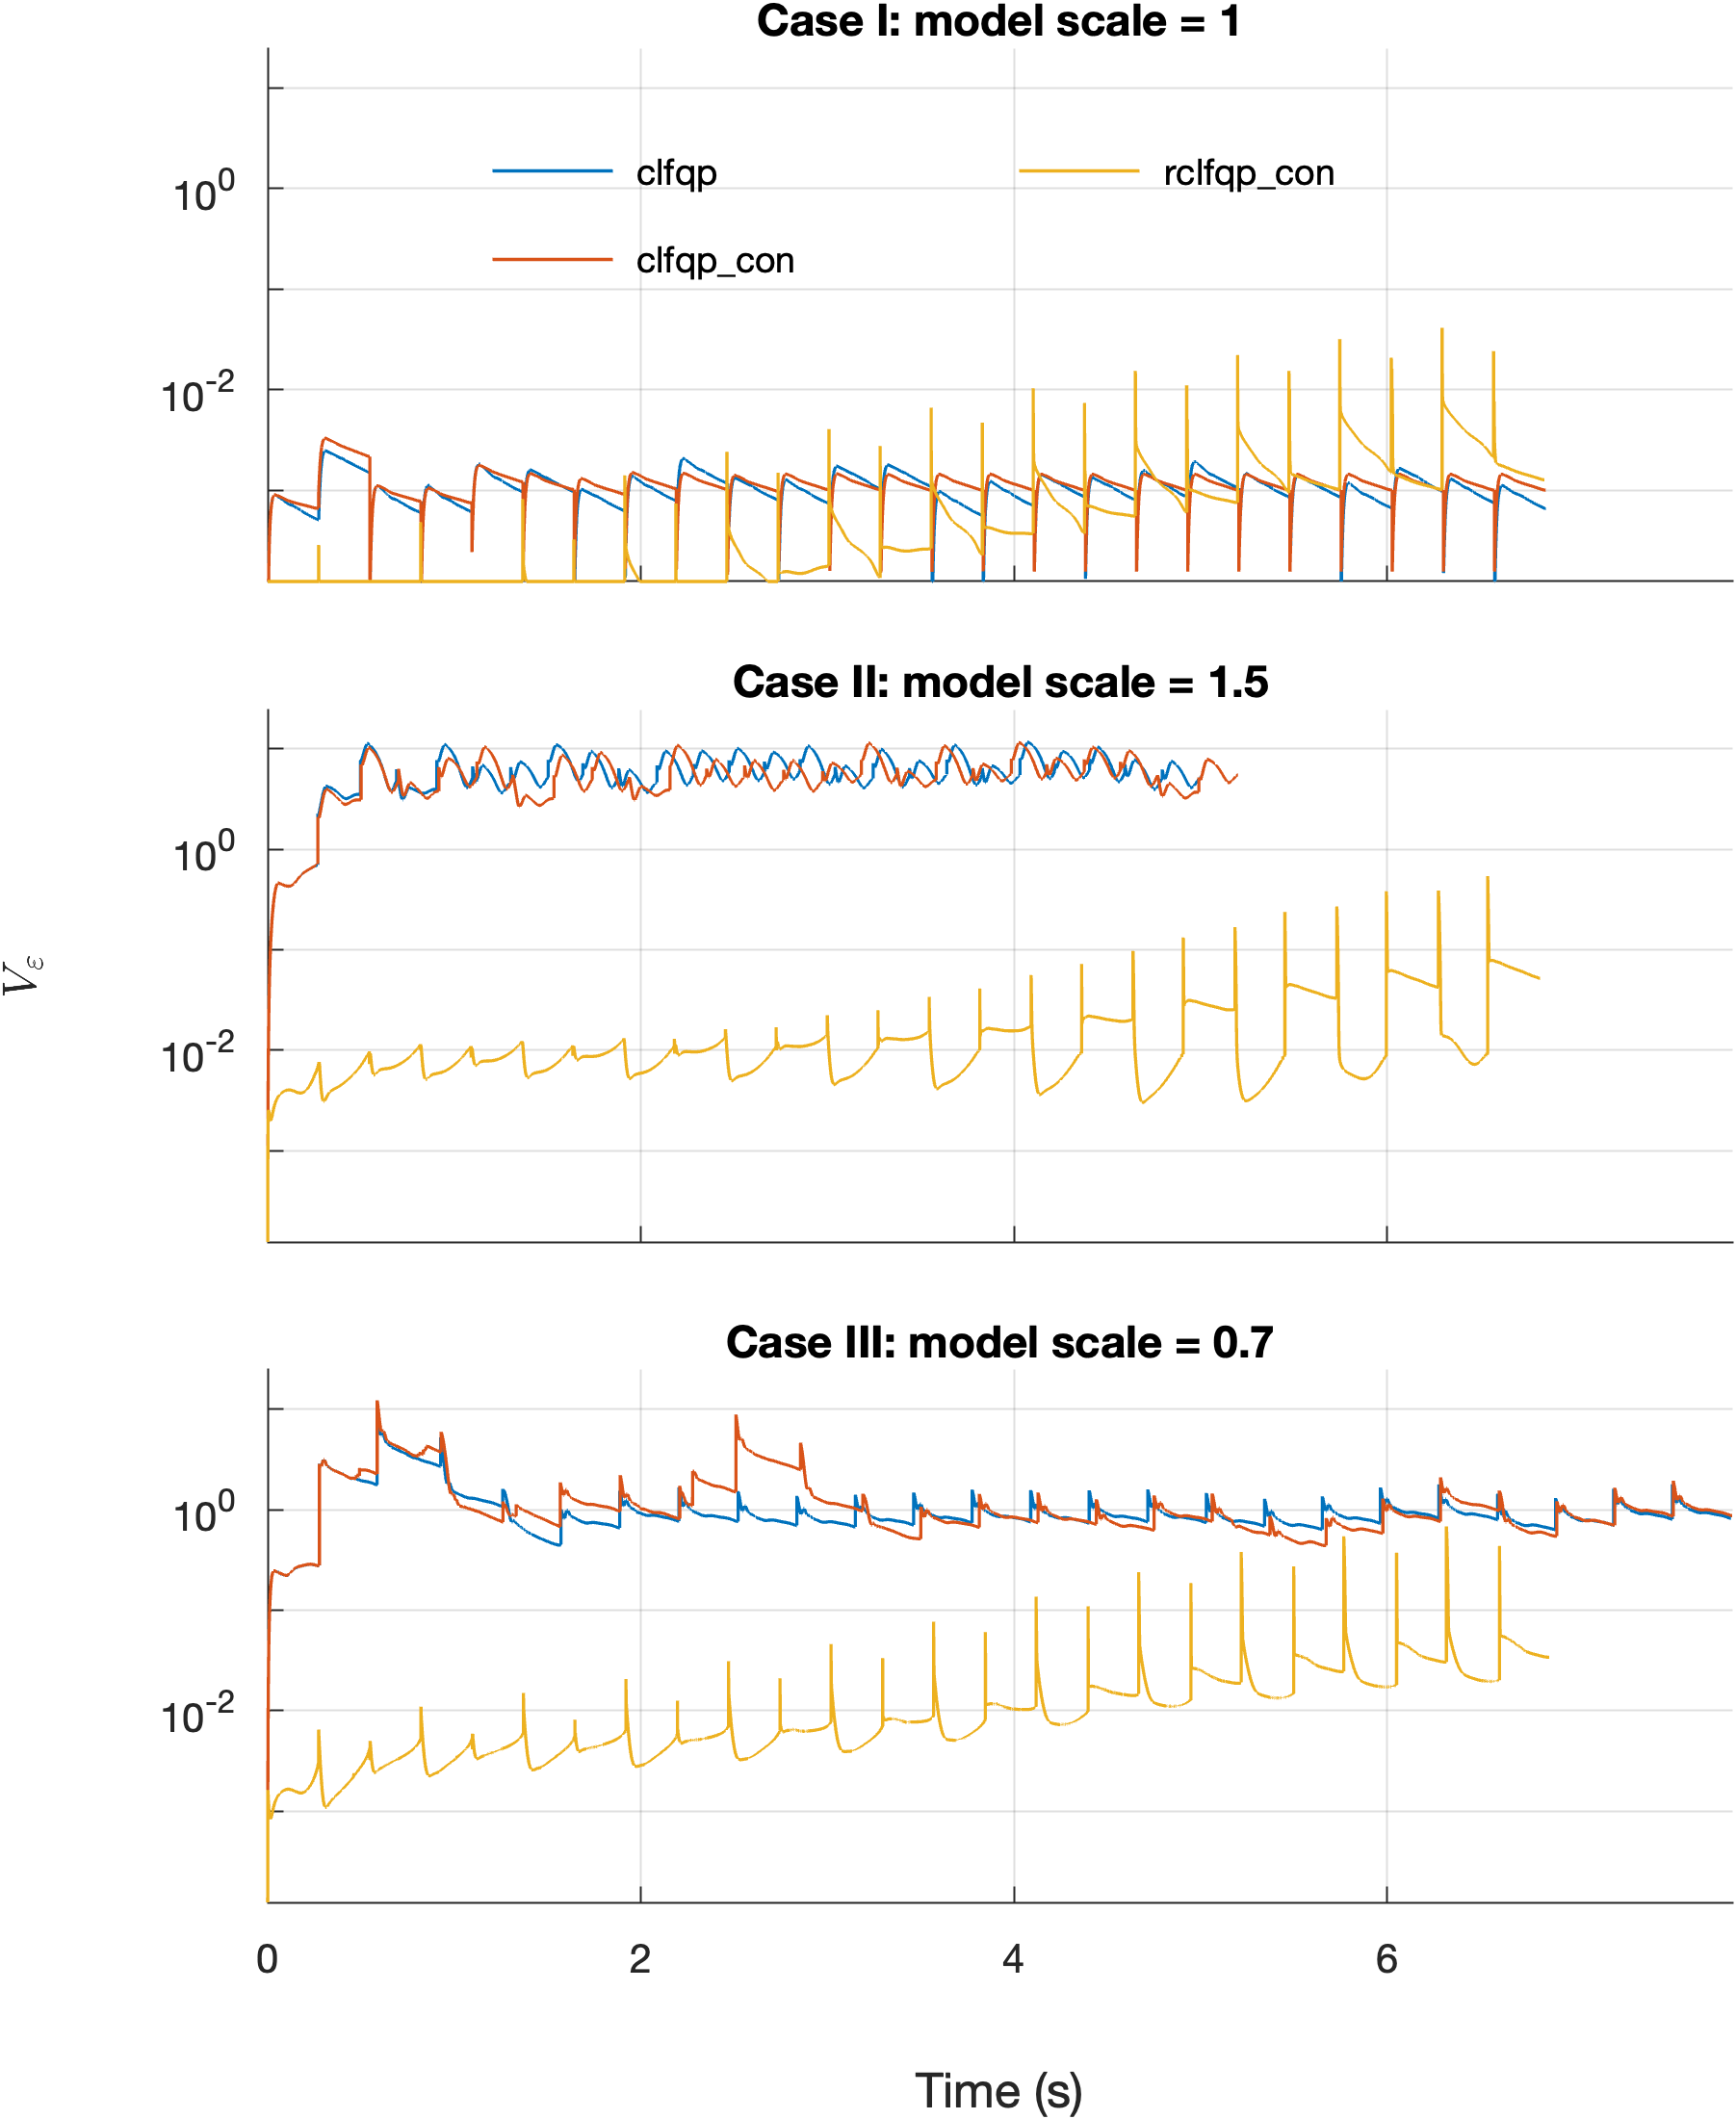
\includegraphics[width=\columnwidth]{ch4_robust_clf.png}
    \caption{مقدار $V_\varepsilon$ در $25$ گام روی مقیاس لگاریتمی، یک قاب برای هر
    حالت. تحت هر دو اغتشاش، قانون مقاوم (زرد) حدود دو مرتبه بزرگی زیر هر دو
    کنترل‌کننده مبنا آغاز می‌کند و در گام $25$ هنوز $4$ تا $14$ برابر پایین‌تر است؛
    این همان تقابل تذکر~\en{4.6} است. اما قله هر گام آن در طول اجرا \emph{رشد}
    می‌کند.}
    \label{fig:robustV}
\end{figure}

\subsection{رشد خطا و فلات آن}
قله گام‌به‌گام $V$ برای قانون مقاوم در طول $25$ گام رشد می‌کند: با مدل کامل از
$4.9\times10^{-5}$ به $0.229$، یعنی نزدیک به $4700$ برابر (شکل~\ref{fig:robustV}).
این رشد در $\varepsilon=0.20$ نیز با قیدها، جعبه و $D_2=0$ باقی می‌ماند و تنها با
$D_1=0$ ناپدید می‌شود ($4.4\times10^{-4}$ به $8.7\times10^{-4}$، و بیشینه
$\|\eta\|$ از $2.85$ به $0.26$)، پس از خودِ جمله مقاوم ناشی می‌شود. بدون لایه مرزی
هم ناپدید می‌شود، اما آن اجرا \textbf{هیچ گام معتبری} ندارد: قانون دقیق می‌لرزد و
پا را از زمین می‌کند، پس حذف لایه درمان نیست. دینامیک صفر گام پایدار است
($\delta^2_{\mathrm{zero}}=0.746$) و علت نیست. در $\varepsilon=0.35$ همین رشد ربات
را در گام $21$ حالت \en{I} ساقط می‌کرد؛ در $0.20$ هر $25$ گام کامل و معتبرند، پس
شدت آن به $\varepsilon$ وابسته است، اما سازوکارش نه.

فراتر از افق $25$ گام، این رشد در حدود $35$ گام روی یک فلات کران‌دار می‌نشیند و
ربات با سرعت اسمی راه می‌رود؛ هیچ حالتی سقوط نمی‌کند، اما فلات در دو حالت
\emph{بالاتر} از آستانه تماس است: در $\times1$ لغزش از گام $35$ و در $\times0.7$ از
گام $6$ آغاز می‌شود (جدول~\ref{tab:plateau}).

\begin{table}[H]
    \centering
    \caption{قانون مقاوم فراتر از $25$ گام، با جعبه $556$ نیوتن‌متری ($731$ در
    $\times3$): فلات (میانگین قله گام‌به‌گام $V$ و بیشینه $\|\eta\|$)، گام استقرار،
    سرعت ده گام آخر (سرعت اسمی $1.563$ متر بر ثانیه) و گام‌های معتبر}
    \label{tab:plateau}
    \small
    \begin{tabular}{lccccc}
        \toprule
        حالت & فلات $V$ & $\|\eta\|$ & استقرار & سرعت & معتبر \\
        \midrule
        $\times1$ ($60$ گام) & $2.2$ & $9.05$ & $\sim35$ & $1.557$ & $34$ \\
        $\times0.7$ ($60$ گام) & $0.68$ تا $0.73$ & $5.27$ & $\sim35$ & $1.552$ & $5$ \\
        $\times1.5$ ($60$ گام) & $0.86$ تا $0.88$ & $5.64$ & $\sim35$ & $1.575$ & $58$ \\
        $\times3$ ($120$ گام) & $0.16$ تا $0.17$ & $1.88$ & $\sim10$ & $1.541$ & $120$ \\
        \bottomrule
    \end{tabular}
\end{table}

بنابراین رانش، گذرایی به سوی کران‌داری نهایی است و نه واگرایی. اما سه نتیجه از آن
پیداست. نخست، تذکر~\en{4.6} در افق بلند برقرار نیست، و با جعبه یکسان حتی ترتیب آن
هم به هم می‌خورد: خطای پایا دیگر با اغتشاش رشد نمی‌کند، بلکه بزرگ‌ترین مقدارش
درست در حالت \en{I} رخ می‌دهد ($9.05$ در برابر $5.27$، $5.64$ و $1.88$). دوم، بهای
مقاومت با مدل کامل یک خطای پایاست، و این بها اکنون آشکارتر است: قانون مقاوم در
حالت \en{I} روی $\|\eta\|\approx9$ و فلات $V=2.2$ می‌نشیند، در برابر $0.25$ برای
\en{A}. مزیت تذکر~\en{4.7}\md{}ردیابی دقیق‌تر وقتی بدترین حالت رخ نمی‌دهد\md{}تا گام
$5$ برقرار است، تا گام $10$ از دست می‌رود و در $60$ گام بازنمی‌گردد.

سوم و مهم‌تر از هر دو: \textbf{فلات، راه‌رفتن معتبر نیست}. با جعبه بزرگ‌تر، قانون
مقاوم اجازه دارد گشتاور بیشتری بکشد و خطای پایای بزرگ‌تری را تحمل کند، و همان خطا
اصطکاک لازم را از $\mu_s=0.4$ عبور می‌دهد: در $\times1$ از گام $35$ و در $\times0.7$
از گام $6$. تنها $\times3$\md{}که جعبه‌اش نسبت به وزنش تنگ‌تر است\md{}هر $120$ گام را
معتبر می‌رود. پس «هیچ حالتی سقوط نمی‌کند» در افق بلند، حکمی درباره شبیه‌ساز است و نه
درباره ربات.

\subsection{حالت \en{IV}: سه برابر جرم}
حالت \en{IV} با کرانه‌های اندازه‌گیری‌شده در مقیاس $3$ اجرا می‌شود
($D_1=434.2$ و $D_2=0.800$، در برابر $\|\Delta_2\|=2/3$ دقیق) و جعبه $731$
نیوتن‌متری، یعنی رده عمل‌گر همین حالت؛ ادغام کرانه‌های آن در کرانه‌های حالت‌های
\en{I} تا \en{III}، قانون مقاوم را برای اغتشاشی تنظیم می‌کرد که آن حالت‌ها هرگز با
آن روبه‌رو نمی‌شوند.

\begin{table}[H]
    \centering
    \caption{حالت \en{IV}، مقیاس جرم $\times3$، در $25$ گام، با جعبه $731$
    نیوتن‌متری. $^{\dagger}$ شماره گامی که ربات در آن سقوط کرد.}
    \label{tab:case4}
    \small
    \begin{tabular}{lc}
        \toprule
        کنترل‌کننده & گام $|$ معتبر $|$ $\|\eta\|$ $|$ نیروی عمودی \\
        \midrule
        \en{A}\ \ \code{clfqp}       & $\mathbf{4}^{\dagger}\;|\;2\;|\;19.6\;|\;5$ \\
        \en{B}\ \ \code{clfqp\_con}   & $\mathbf{3}^{\dagger}\;|\;2\;|\;17.5\;|\;528$ \\
        \en{C}\ \ \code{rclfqp\_con}  & $25\;|\;\mathbf{25}\;|\;\mathbf{1.89}\;|\;96$ \\
        \bottomrule
    \end{tabular}
\end{table}

کنترل‌کننده‌های \en{A} و \en{B} همان‌گونه که متن مرجع می‌گوید شکست می‌خورند، و با
جعبه یکسان زودتر: \en{A} سه گام با مدت‌هایی که فرو می‌ریزند می‌رود و گام چهارمش
کوتاه‌تر از کف $0.15$ متری است، و \en{B} در گام سوم پای آزاد را اصلاً از زمین بلند
نمی‌کند. هر دو تنها $2$ گام معتبر دارند. قانون مقاوم با افتی اندک راه می‌رود و هر
$25$ گامش معتبر است: خطای $1.89$ در برابر $2.85$ در حالت \en{I}، نیروی عمودی دست‌کم
$96$ نیوتن، اصطکاک لازم حداکثر $0.36$، و بیشینه گشتاور که روی جعبه $731$
نیوتن‌متری می‌نشیند (شکل~\ref{fig:case4}).

\begin{figure}[t]
    \centering
    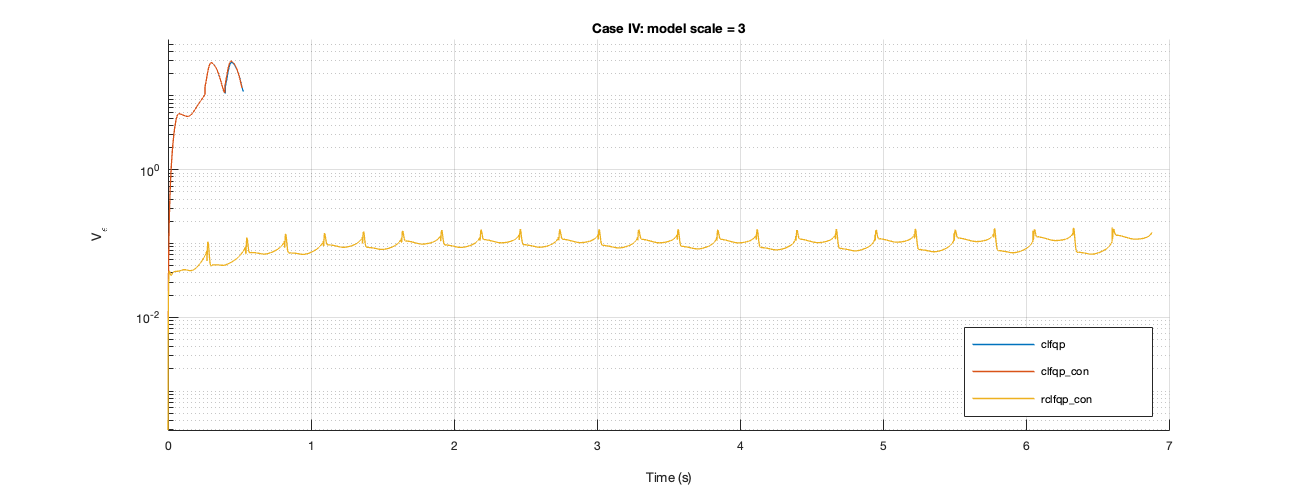
\includegraphics[width=\columnwidth]{ch4_case4_clf.png}
    \caption{حالت \en{IV}. هر دو کنترل‌کننده مبنا ظرف نیم ثانیه از قاب بیرون
    می‌روند و با سقوط پایان می‌یابند؛ قانون مقاوم $V_\varepsilon$ را نزدیک $0.1$ با
    جهشی کوچک در هر برخورد پا نگه می‌دارد.}
    \label{fig:case4}
\end{figure}

\textbf{آنچه بازتولید نمی‌شود: کند شدن تا توقف کامل.} متن مرجع گزارش می‌کند که
راه‌رفتن در حالت \en{IV} «پس از چند گام تا توقف کامل کند می‌شود» و آن را به مداری
ناپایدار نسبت می‌دهد. در اینجا \en{C} یک اجرای $120$ گامی را با $1.541$ متر بر
ثانیه\md{}یعنی $1.4$ درصد زیر سرعت اسمی\md{}و با هر $120$ گام معتبر کامل می‌کند. اگر
حالت \en{IV} متن مرجع نیز مقیاس یکنواخت جرم باشد\md{}که این گزارش جداگانه تصدیق
نکرده است\md{}آن توضیح روی این مدل نمی‌تواند برقرار باشد: مقیاس یکنواخت جرم دینامیک
صفر هیبریدی را دقیقاً ناوردا می‌گذارد و دینامیک صفر این گام پایدار است. با جعبه
$731$ نیوتن‌متری، خطا نیز فراتر از گام $25$ رها نمی‌شود و روی $\|\eta\|\approx1.9$
و فلات $V\approx0.17$ می‌ماند\md{}کم‌ترین فلات میان چهار حالت.

\begin{figure}[t]
    \centering
    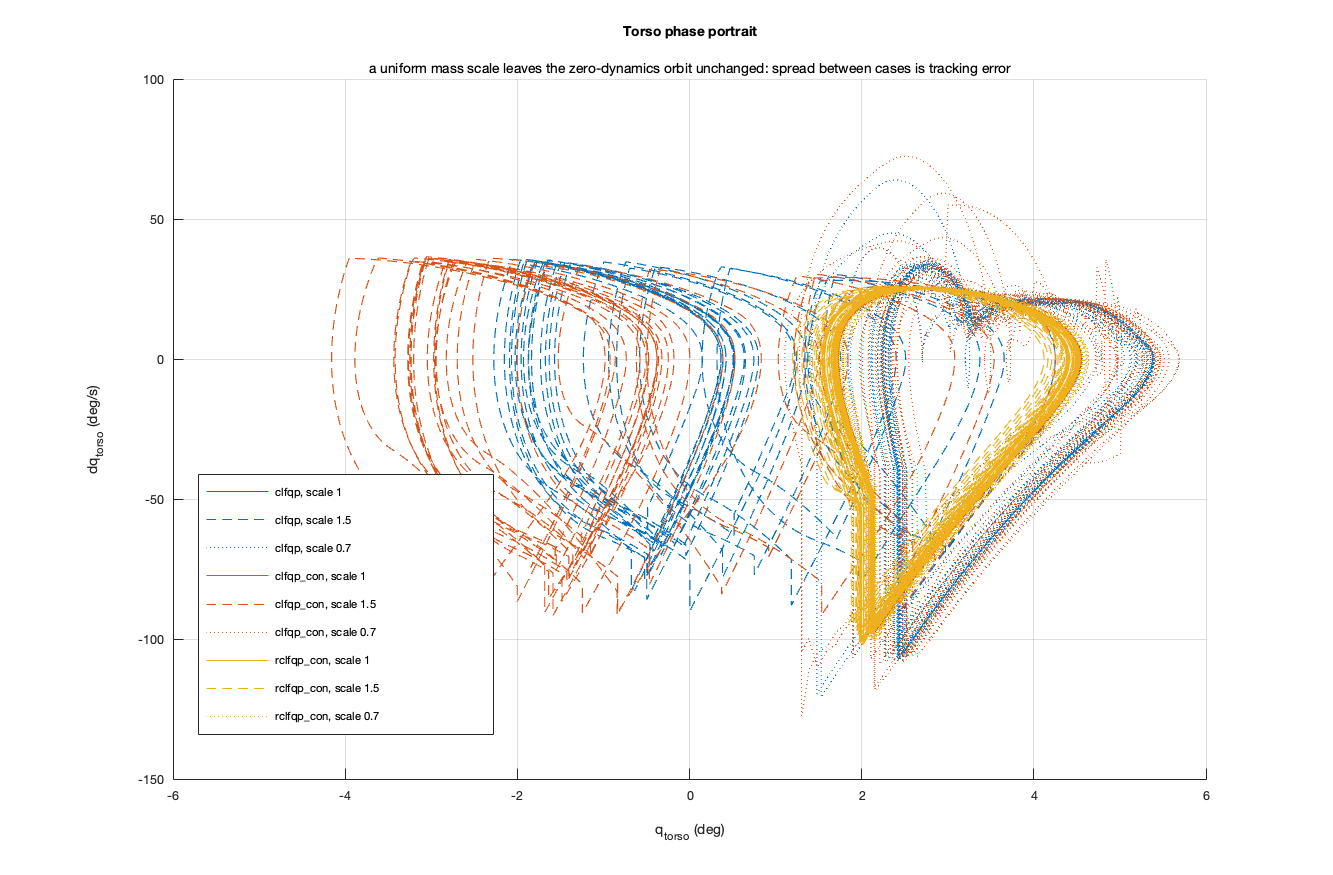
\includegraphics[width=\columnwidth]{ch4_robust_torso.png}
    \caption{تصویر فاز تنه در $25$ گام، همتای شکل~\en{4.6}. متن مرجع سه مدار متفاوت را
    توصیف می‌کند؛ اینجا سه حالت قانون مقاوم (زرد) روی هم می‌افتند و باید بیفتند:
    مقیاس یکنواخت جرم دینامیک صفر را ناوردا می‌گذارد، پس کنترل‌کننده‌ای که قیدهای
    مجازی را اعمال کند، مدار اسمی را برای هر $s$ طی می‌کند. جابه‌جایی مدارهای
    کنترل‌کننده‌های مبنا، تا حدود $6$ درجه در $\times1.5$، خطای ردیابی است و نه مداری
    تازه.}
    \label{fig:torso}
\end{figure}

% =====================================================================
\section{کنترل تطبیقی \Lone{} و چهار اصلاح}
% =====================================================================
قانون مقاوم بهای بدترین حالت را می‌پردازد، چه آن حالت رخ دهد و چه ندهد. کنترل
$\mathcal{L}_1$ عدم قطعیت را تخمین می‌زند و خنثی می‌کند، پس مدل کامل هزینه‌ای
ندارد \cite{hovakimyan2010l1}. ورودی اعمال‌شده به صورت $\mu=\mu_1+\mu_2$ تقسیم
می‌شود: $\mu_1$ خودِ \en{CLF-QP} فصل سوم است\md{}یک مدل مرجع غیرخطی بدون شکل
بسته\md{}و $\mu_2=-C(s)\hat\theta$ تخمین $\hat\theta=\hat\alpha\|\eta\|+\hat\beta$ را
خنثی می‌کند. برخلاف فصل سوم، کنترل‌کننده حالت دارد: بیست درایه شامل پیش‌بین
حالت، دو تخمین و خروجی فیلتر.

اجرای این کنترل‌کننده به صورتی که در بخش~\en{4.2} نوشته شده، ادعای خود را روی این
ربات بازتولید نمی‌کند: در $25$ گام تحت هر دو اغتشاش بهتر از مدل مرجع خود ردیابی
نمی‌کند، در $\times1.5$ در گام $14$ سقوط می‌کند، و در $11$ تا $14$ درصد نمونه‌ها نیاز
دارد زمین پا را به پایین بکشد. چهار تغییر آن را پایدار می‌کنند؛ هر کدام گزینه‌ای در
\code{p.l1} است و صورت متن مرجع تنها یک تنظیم فاصله دارد.

پیش از آنکه این چهار تغییر شمرده شوند، باید صادقانه نامگذاری شوند. پیش‌بینی که با
ورودی اعمال‌شده رانده می‌شود، پیشروی نمونه‌برداری‌شده سازگار، قیدهایی روی گشتاور
\emph{کل} به‌جای تنها $\mu_1$، و یک قانون تطبیق نرمال‌شده\md{}این‌ها روی هم
\textbf{کنترل‌کننده دیگری می‌سازند و نه $\mathcal{L}_1$ متن مرجع با چند اصلاح}. سه
تغییر نخست ساختار پیش‌بین و مجموعه شدنی را عوض می‌کنند و چهارمی خودِ قانون تطبیق را.
گفتن این نکته فصل را قوی‌تر می‌کند و نه ضعیف‌تر: آنچه در ادامه سنجیده می‌شود
کارایی این طراحی است، و گزاره درباره متن مرجع تنها این است که صورت منتشرشده آن روی
این ربات و در این نرخ نمونه‌برداری کار نمی‌کند.

\textbf{۱. پیش‌بین با ورودی دریافتی ربات رانده می‌شود.} پیش‌بین متن مرجع (\en{4.19})
نسخه‌ای از مدل مرجع را با \en{QP} دومی روی $\hat\eta$ اجرا می‌کند. گذر از (\en{4.24}) به
(\en{4.28}) نیاز دارد که $\hat\mu_1(\hat\eta)-\mu_1(\eta)$ مقدار $P_\varepsilon$ را در
امتداد $\tilde\eta$ کاهش دهد، اما دو \en{QP} تنها کاهش را در امتداد $\eta$ و
$\hat\eta$ به‌طور جداگانه تضمین می‌کنند و قانون کمینه‌نرم غیرخطی است. این ناهمخوانی
درست مانند خطای مدل $\tilde\eta$ را می‌راند و تطبیق آن را جذب می‌کند: در
$\varepsilon=0.35$، $\hat\theta$ از $\theta$ سه تا پنج برابر فراتر رفت. پیش‌بین
استاندارد $\mathcal{L}_1$ از ورودی واقعاً دریافتی ربات استفاده می‌کند:
\begin{equation}
    \dot{\hat\eta} = F\eta + G(\mu+\hat\theta) - a(\hat\eta-\eta)
    \;\Rightarrow\;
    \dot{\tilde\eta} = -a\tilde\eta + G\tilde\theta
    \label{eq:plant}
\end{equation}
به‌طور دقیق و بدون حضور مدل مرجع؛ پس $P=I$، قانون روی خطای پیش‌بینی سرعت تطبیق
می‌یابد، کانال $\hat\beta$ حلقه $s^2+as+\Gamma$ را می‌بندد، و \en{QP} دوم حذف
می‌شود.

\textbf{۲. پیشروی نمونه‌برداری‌شده ورودی‌های ربات را می‌بیند.} پیشروی متن مرجع،
$\eta$ را در هر دوره $1$ میلی‌ثانیه‌ای ثابت نگه می‌داشت و $\mu_2$ را همراه فیلتر
حرکت می‌داد؛ ربات عکس آن را می‌دید. اکنون پیشروی $\mu$ اعمال‌شده را نگه می‌دارد و
$\eta$ را در هر دو سر دوره می‌خواند، که علّی می‌ماند چون $\eta$ پیش از محاسبه کنترل
بعدی در $t_{k+1}$ نمونه‌برداری می‌شود. روی یک انتگرال‌گیر دوگانه ردیاب، این روش
$\theta$ را با خطای نسبی $10^{-15}$ تخمین می‌زند، در حالی که ثابت نگه‌داشتن $\eta$
سوگیری $2.5$ درصدی بر جا می‌گذارد. پس از هر دوره، تخمین‌ها به گوی‌های تصویر
بازگردانده می‌شوند، زیرا تصویر فقط در زمان پیوسته آن‌ها را کران‌دار می‌کند و پیش
از این کار $\hat\theta$ یک بار به $10^{7}$ رسید.

\textbf{۳. قانون قیددار گشتاوری را که اعمال می‌کند مقید می‌کند.} بخش~\en{4.2.3} تنها
$\mu_1$ را در جعبه قرار می‌دهد و قید تماسی نمی‌افزاید، پس $\mu_2$ بیرون از هر قیدی به
مفاصل می‌رسد. با \code{p.l1.constrain\_applied}، $\mu_2$ به صورت یک جابه‌جایی معلوم
وارد \en{QP} می‌شود: هزینه و سطر \en{CLF} همچنان روی $\mu_1$ عمل می‌کنند، اما جعبه و
قیدهای اصطکاک و نیروی عمودی گشتاور \emph{کل} را محدود می‌کنند. چون جعبه اکنون کل
ربات را حمل می‌کند، باید سنگین‌ترین حالت پاکت طراحی را بردارد: رباتی $1.5$ برابر
سنگین‌تر تنها برای پیش‌خور $293$ نیوتن‌متر لازم دارد، که رده $556$ نیوتن‌متری آن را
با حاشیه در بر می‌گیرد؛ جعبه $65$ نیوتن‌متری متن مرجع حتی پیش‌خور اسمی را هم
نمی‌پوشاند.

\textbf{۴. قانون تطبیق برای حلقه نمونه‌برداری‌شده نرمال می‌شود.} حلقه از خطای
پیش‌بینی به تخمین‌ها با بسامد تقریبی $\sqrt{\Gamma+\Gamma_\alpha\|\eta\|^2}$ رادیان
بر ثانیه کار می‌کند، یعنی با بدتر شدن ردیابی \emph{تندتر} می‌شود. پس از یک برخورد
نامناسب پا، در $\|\eta\|=13$، به $4.1$ رادیان در هر نمونه $1$ میلی‌ثانیه‌ای می‌رسد،
تندتر از آنچه کنترل‌کننده‌ای با نرخ $1$ کیلوهرتز بتواند محقق کند. بنابراین هر دو
قانون تطبیق بر
\begin{equation}
    m^2 = \max\!\Big(1,\ \frac{\Gamma+\Gamma_\alpha\|\eta\|^2}{(\rho/\Delta t)^2}\Big),
    \qquad \rho = 0.75
    \label{eq:norm}
\end{equation}
تقسیم می‌شوند (\code{p.l1.normalized\_rate})، که حلقه را در $\rho$ رادیان بر نمونه
نگه می‌دارد و هر جا حلقه کندتر است قانون را دست‌نخورده می‌گذارد؛ خودِ $\hat\theta$
تغییر نمی‌کند. استدلال لیاپانوف به شکلی ضعیف‌تر باقی می‌ماند: با وزن $1/m^2$ روی
خطای پیش‌بینی، جملات متقاطع همچنان حذف می‌شوند، اما کران خطای پیش‌بینی به ضریب
$m$ گشاد می‌شود و تنها تا وقتی برقرار است که $m^2$ کندتر از $e^{-2at}$ کاهش یابد،
شرطی که برخورد پا می‌تواند نقض کند \cite{ioannou1996robust}. بخش~\ref{sec:long}
توضیح می‌دهد چرا این اصلاح لازم است و چرا $\rho=0.75$.

\begin{table}[H]
    \centering
    \caption{کنترل‌کننده $\mathcal{L}_1$ آن‌گونه که اجرا شد}
    \label{tab:l1params}
    \small
    \begin{tabular}{lc}
        \toprule
        جزء & مقدار \\
        \midrule
        پیش‌بین، نرخ $a$ & مبتنی بر ورودی ربات، $800$ \\
        بهره تطبیق $\Gamma=\Gamma_\alpha$ & $10^5$ \\
        گوی‌های تصویر & $\|\hat\alpha\|\le200,\ \|\hat\beta\|\le400$ \\
        فیلتر $C(s)$ & $\omega_c=150$ رادیان بر ثانیه \\
        جعبه گشتاور & $244\times\max(1,s)$ نیوتن‌متر \\
        نرخ نرمال‌سازی $\rho$ & $0.75$ رادیان بر نمونه \\
        کنترل و پیشروی & $1$ کیلوهرتز، رونگه-کوتا \\
        \bottomrule
    \end{tabular}
\end{table}

در این تنظیم (جدول~\ref{tab:l1params})، میرایی $a/(2\sqrt\Gamma)$ برابر $1.26$ است؛
پهنای باند کانال $\hat\beta$، یعنی $\sqrt\Gamma=316$ رادیان بر ثانیه، بالاتر از
$150$ رادیان بر ثانیه فیلتر است (در $\Gamma=10^4$ پایین‌تر بود)؛ جعبه $1.25$ برابر
بیشینه $195$ نیوتن‌متری خودِ گام است، زیرا جعبه‌ای بدون حاشیه \en{QP} را گرسنه و
تطبیق را واگرا می‌کند؛ و پیشروی با رونگه-کوتا انجام می‌شود، چون روش اویلر در
حلقه‌ای با این سختی می‌تواند انرژی بیفزاید و به شکل «ناپایداری $\mathcal{L}_1$»
دیده شود.

% =====================================================================
\section{نتایج \Lone{} در مقیاس‌های جرم}
% =====================================================================
سه کنترل‌کننده بخش~\en{4.2.4} مقایسه می‌شوند: \en{A} همان \en{CLF-QP}، \en{B}
کنترل $\mathcal{L}_1$ روی آن، و \en{C} کنترل $\mathcal{L}_1$ با جعبه گشتاور و قیدهای
تماس (جدول~\ref{tab:l1}).

\begin{table*}[!t]
    \centering
    \caption{بخش~\en{4.2.4}: کنترل $\mathcal{L}_1$ در برابر مدل مرجع خود در $25$ گام،
    همه با جعبه $556$ نیوتن‌متری روی گشتاور \textbf{کل}. هر خانه:
    تعداد گام $|$ گام‌های معتبر $|$ بیشینه $\|\eta\|$ $|$ کمینه نیروی عمودی واقعی.
    سطر آخر صورت متن مرجع است (پیش‌بین متن مرجع، $\Gamma=10^4$، جعبه تنها روی
    $\mu_1$ و از این رو با قاعده جعبه قدیم اندازه‌گیری شده).
    $^{\dagger}$ شماره گامی که ربات در آن سقوط کرد.}
    \label{tab:l1}
    \small
    \begin{tabular}{lccc}
        \toprule
        کنترل‌کننده & حالت \en{I}، $\times1$ & حالت \en{II}، $\times1.5$ & حالت \en{III}، $\times0.7$ \\
        \midrule
        \en{A}\ \ \code{clfqp}  & \rcv{25}{1}{0.25}{26} & \rcv{25}{\mathbf{0}}{16.5}{\mathbf{-179}} & \rcv{25}{\mathbf{0}}{14.5}{\mathbf{-1734}} \\
        \en{B}\ \ \code{l1}     & \rcv{25}{25}{0.14}{50} & \rcv{25}{\mathbf{0}}{2.37}{\mathbf{-227}}  & \rcv{25}{\mathbf{0}}{4.34}{\mathbf{-220}} \\
        \en{C}\ \ \code{l1\_con} & \rcv{25}{25}{0.15}{50} & \rcv{25}{25}{6.10}{91}            & \rcv{25}{\mathbf{0}}{5.89}{23} \\
        \midrule
        \en{C}، صورت متن مرجع & \rc{25}{0.38}{49} & \fallc{14}{18.7}{-978} & \rc{25}{14.5}{-1403} \\
        \bottomrule
    \end{tabular}
\end{table*}

\textbf{با مدل کامل، $\mathcal{L}_1$ دست‌کم به خوبی \en{CLF-QP} است}: بیشینه خطای
$0.14$ در برابر $0.25$ و مقدار \en{CLF} میان برخوردها حدود چهار برابر کمتر. تخمین
کاملاً صفر نیست ($\|\hat\theta\|\le9$)، زیرا نگهداری $1$ کیلوهرتزی شتاب خروجی را درون
هر دوره منحرف می‌کند و $\mathcal{L}_1$ بخشی از این خطای میان‌نمونه‌ای را خنثی
می‌کند؛ در زمان پیوسته این همانی دقیق است و مجموعه آزمون آن را تا دقت ماشین تصدیق
می‌کند.

\textbf{تحت هر دو اغتشاش گام‌ها کامل می‌شوند، اما تنها یکی از دو اغتشاش معتبر
است.} هر دو قانون همه $25$ گام را با خطای $2.4$ تا $6.1$ در برابر $14.5$ تا $16.5$
برای مبنا طی می‌کنند و زمان گام را نزدیک مقدار اسمی نگه می‌دارند، و قله گام‌به‌گام
\en{CLF} برای \code{l1\_con} تقریباً ثابت می‌ماند، در حالی که قله قانون مقاوم رشد
می‌کند (شکل~\ref{fig:l1V}). در $\times1.5$ این تصویر پابرجاست: \code{l1\_con} هر
$25$ گام را \textbf{معتبر} می‌رود، نیروی عمودی دست‌کم $91$ نیوتن و اصطکاک لازم
حداکثر $0.27$.

اما در $\times0.7$ هیچ‌یک از سه قانون حتی یک گام معتبر ندارد. \code{clfqp} و
\code{l1} نیروی عمودی را منفی می‌کنند ($-1734$ و $-220$ نیوتن)، و \code{l1\_con} با
آنکه نیروی عمودی‌اش دست‌کم $23$ نیوتن می‌ماند\md{}یعنی قیدهای تماس روی مدل اسمی کار
خود را می‌کنند\md{}اصطکاکی تا $1.58$، نزدیک چهار برابر $\mu_s=0.4$، می‌طلبد. قید
نوشته‌شده روی مدل \emph{اسمی} نمی‌تواند اصطکاک مدل \emph{واقعی} را کران‌دار کند، و
در سبک‌ترین حالت این شکاف تعیین‌کننده است. \textbf{پس ادعای «پایداری تحت هر دو
اغتشاش» تنها برای $\times1.5$ برقرار می‌ماند.}

تخمین همچنان عدم قطعیت را اندازه می‌گیرد: با پیش‌بین ورودی-گیاه، میانه
$\|\hat\theta\|/\|\theta\|$ در $\times0.7$ برابر $0.92$ و در $\times1.5$ برابر
$0.98$ است (بیشینه نسبت $1.29$ و $1.01$)، در حالی که در صورت متن مرجع و در همان
$\varepsilon=0.20$ بیشینه نسبت به $7.2$ و $2.0$ می‌رسد
(شکل~\ref{fig:l1theta}).

\begin{figure}[t]
    \centering
    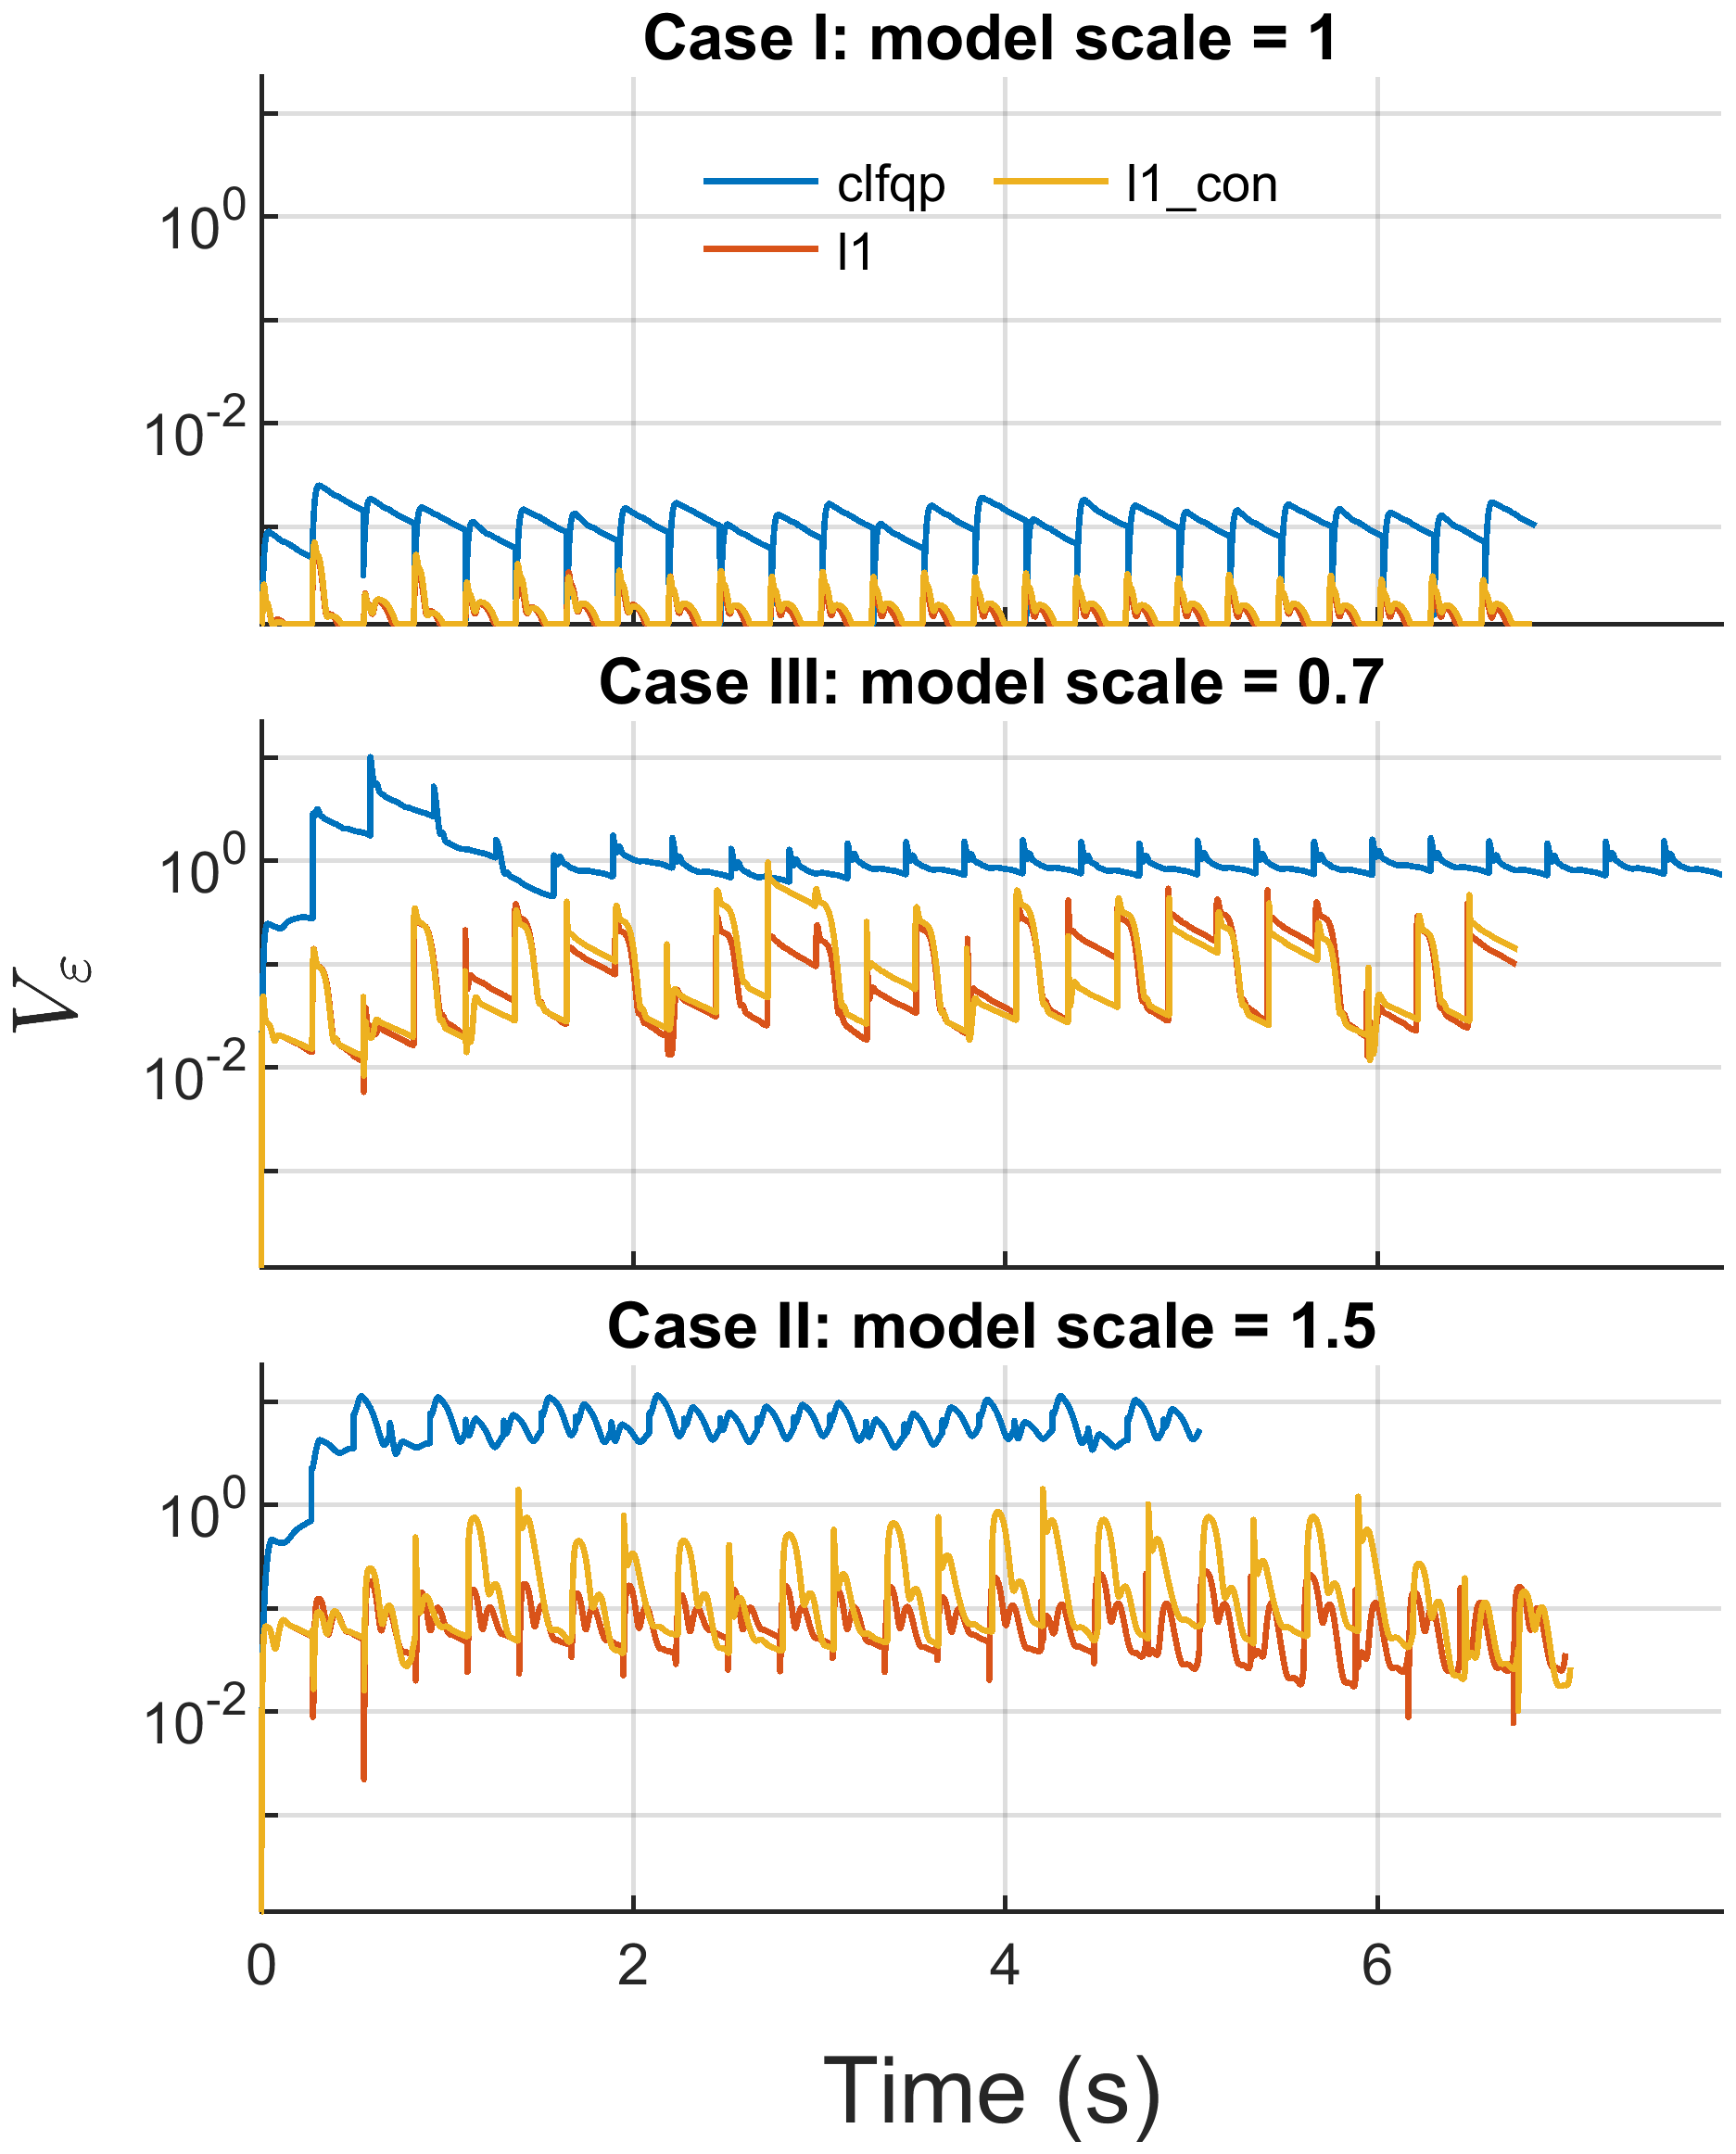
\includegraphics[width=\columnwidth]{ch4_l1_clf.png}
    \caption{$V_\varepsilon$ برای \en{CLF-QP} (آبی) و هر دو قانون $\mathcal{L}_1$.
    در هر دو قاب اغتشاش‌دار، منحنی‌های $\mathcal{L}_1$ یک تا دو مرتبه بزرگی زیر مبنا
    می‌نشینند و از گام‌های نخست ثابت می‌مانند؛ با مدل کامل نیز پایین‌ترند. قاب‌ها با
    همان شماره‌گذاری جدول~\ref{tab:robust} برچسب خورده‌اند (\en{I} مقیاس $1$،
    \en{II} مقیاس $1.5$، \en{III} مقیاس $0.7$)، هرچند این مجموعه آن‌ها را به ترتیب
    $1$، $0.7$، $1.5$ اجرا می‌کند.}
    \label{fig:l1V}
\end{figure}

\begin{figure}[t]
    \centering
    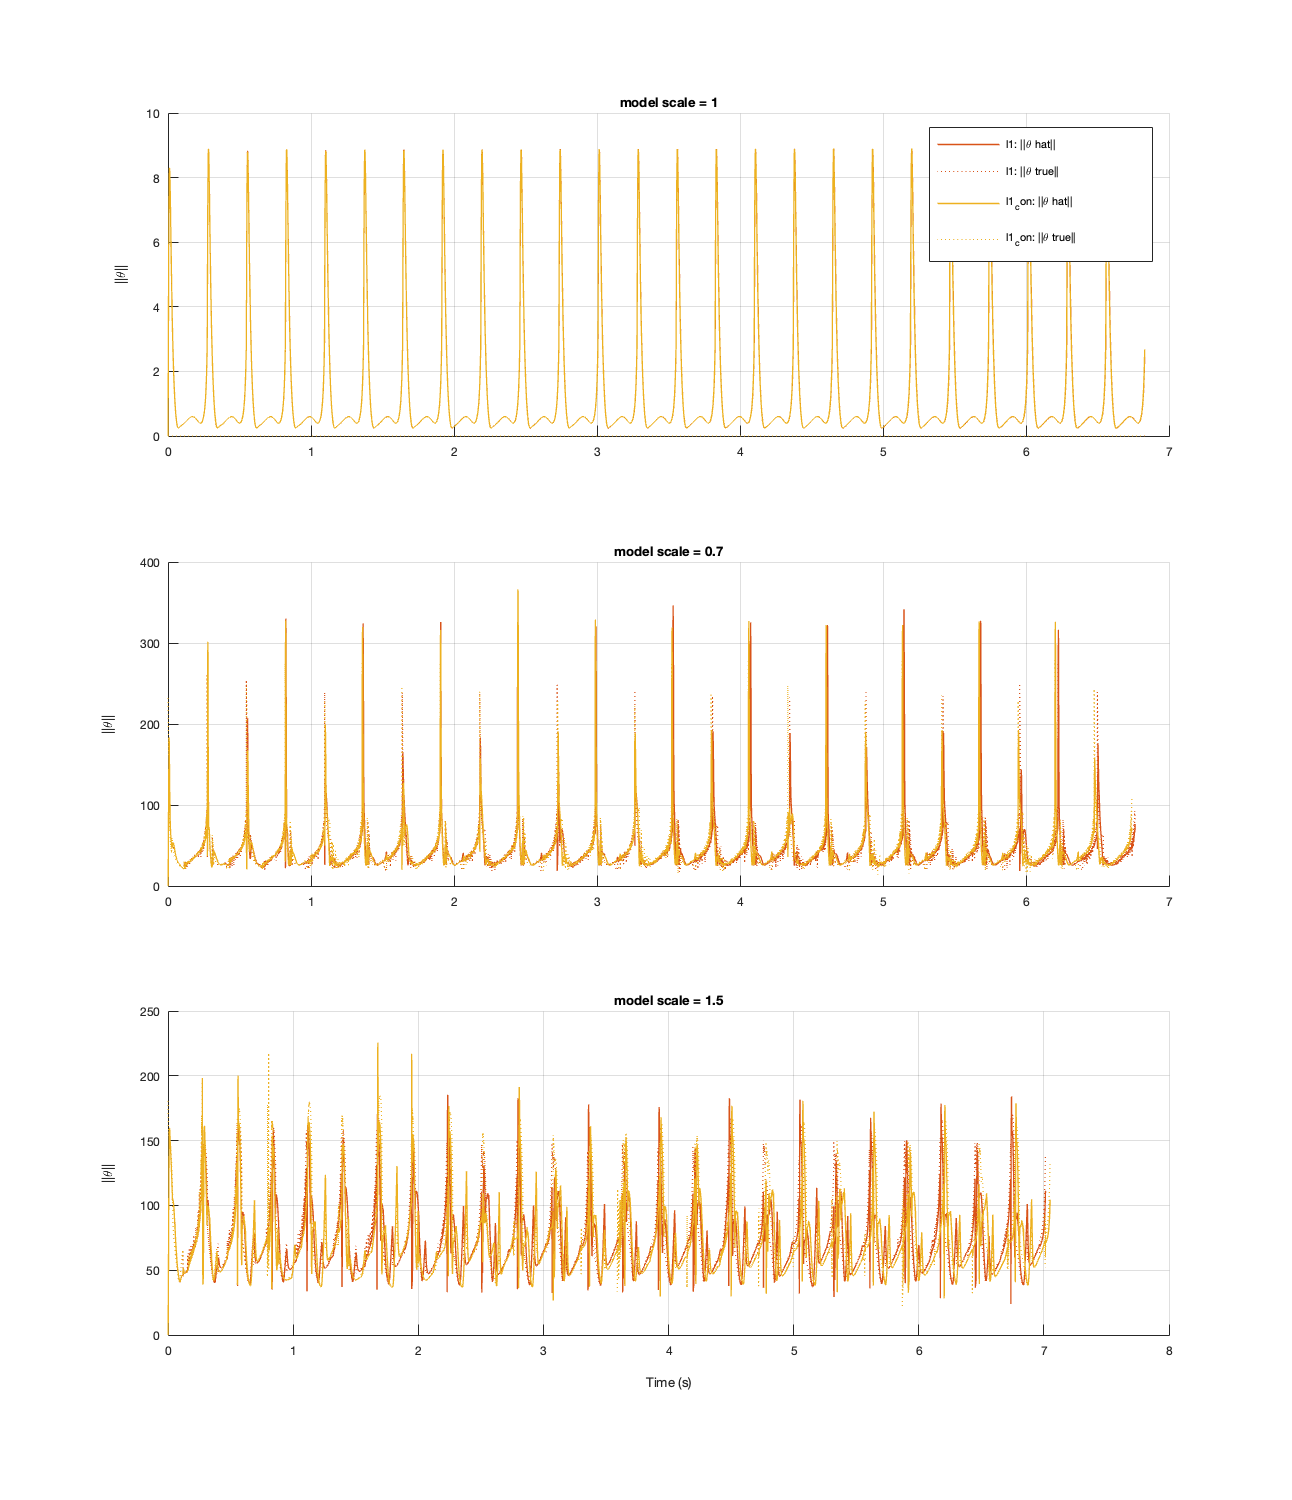
\includegraphics[width=\columnwidth]{ch4_l1_theta.png}
    \caption{$\|\hat\theta\|$ (پیوسته) در برابر $\|\theta\|$ واقعی (نقطه‌چین). با مدل کامل
    $\theta$ صفر است و تخمین در هر برخورد پا به حدود $9$ می‌رسد: همان خطای
    میان‌نمونه‌ای که خنثی می‌کند. تحت هر دو اغتشاش، دو منحنی روی هم می‌افتند.}
    \label{fig:l1theta}
\end{figure}

\textbf{مقیاس $\times1.5$ نزدیک یک لبه است}، پس جاروب نرخ پیش‌بین به‌جای تنها
گزینه برنده گزارش می‌شود (جدول~\ref{tab:rate}). با جعبه یکسان، \code{l1\_con} در
هشت نرخ از ده نرخ هر $25$ گام را معتبر می‌رود و در دو نرخ سقوط می‌کند\md{}$a=700$
با نرمال‌سازی و $a=800$ بدون آن\md{}که هیچ‌یک الگوی یکنوایی نمی‌سازند. نرخ همچنان
ردیابی را تعیین می‌کند ($4.8$ تا $23.3$)، پس نتیجه $\times1.5$ به این تنظیم تعلق
دارد و نه به یک حاشیه اطمینان. \code{l1} بدون قید در \emph{هیچ} نرخی گام معتبری
ندارد؛ آنچه این مقیاس را نگه می‌دارد قیدهای تماس‌اند و نه سرعت پیش‌بین.

\begin{table*}[!t]
    \centering
    \caption{نرخ پیش‌بین $a$ در مقیاس $\times1.5$ با جعبه $556$ نیوتن‌متری: تعداد گام
    $|$ گام‌های معتبر $|$ بیشینه $\|\eta\|$ در $25$ گام. $^{\dagger}$ شماره گامی که
    ربات در آن سقوط کرد.}
    \label{tab:rate}
    \small
    \begin{tabular}{lccccc}
        \toprule
        کنترل‌کننده & $a=500$ & $632$ (بحرانی) & $700$ & $\mathbf{800}$ (پیش‌فرض) & $900$ \\
        \midrule
        \code{l1}      & $25\;|\;0\;|\;11.1$ & $25\;|\;0\;|\;2.43$ & $25\;|\;0\;|\;2.17$ & $25\;|\;0\;|\;2.37$ & $25\;|\;0\;|\;2.64$ \\
        \code{l1\_con} & $25\;|\;25\;|\;5.74$ & $25\;|\;25\;|\;6.04$ & $\mathbf{21}^{\dagger}\;|\;19\;|\;23.3$ & $25\;|\;25\;|\;6.10$ & $25\;|\;25\;|\;4.80$ \\
        \midrule
        \code{l1}، بدون نرمال‌سازی      & $25\;|\;0\;|\;5.92$ & $25\;|\;0\;|\;2.43$ & $25\;|\;0\;|\;2.17$ & $25\;|\;0\;|\;2.37$ & $25\;|\;0\;|\;2.59$ \\
        \code{l1\_con}، بدون نرمال‌سازی & $25\;|\;25\;|\;6.84$ & $25\;|\;25\;|\;5.56$ & $25\;|\;25\;|\;6.00$ & $\mathbf{16}^{\dagger}\;|\;15\;|\;7.55$ & $25\;|\;25\;|\;4.12$ \\
        \bottomrule
    \end{tabular}
\end{table*}

% =====================================================================
\section{بار ناشناخته}
% =====================================================================
ربات باری را روی مفصل ران حمل می‌کند که هیچ کنترل‌کننده‌ای از آن خبر ندارد: در هر
گام به‌طور تصادفی از بازه $0$ تا $70$ کیلوگرم کشیده می‌شود (شکل~\en{4.11}الف متن مرجع)،
یا ثابت در $23$، $35$ و $46$ کیلوگرم است (شکل~\en{4.11}ب). این مقادیر همان $0$ تا $30$ و
$10$، $15$ و $20$ کیلوگرم متن مرجع‌اند که با نسبت جرم این ربات، $74/32$، مقیاس
گرفته‌اند تا سهم هر بار از وزن بدن یکسان بماند.

دو انتخاب طراحی، هر دو اندازه‌گیری‌شده: نخست، \textbf{یک مبنای دوم}؛ افزون بر سه
کنترل‌کننده بخش~\en{4.2.4}، \code{clfqp\_con} با همان جعبه و قیدهای \code{l1\_con} اجرا
می‌شود، زیرا \en{CLF-QP} بدون قید زیر بار $2$ تا $3.5$ برابر گشتاور \code{l1\_con}
مصرف می‌کند و مقایسه تنها با آن نمی‌گوید کار را تطبیق انجام می‌دهد یا گشتاور.
دوم، \textbf{جعبه}؛ همان رده عمل‌گر $556$ نیوتن‌متری بخش‌های پیشین، برای همه بارها
و همه کنترل‌کننده‌ها. این عدد یک بار از سنگین‌ترین پیش‌خور پاکت طراحی\md{}که بار
$70$ کیلوگرمی را در بر می‌گیرد\md{}ساخته شده است و نه از باری که هر اجرا حمل می‌کند،
پس برخلاف نسخه پیشین این گزارش، جعبه دیگر دانشی از بار ناشناخته ندارد
(جدول~\ref{tab:loads} اثر هر بار را بر بهره ورودی نشان می‌دهد).

\begin{table}[H]
    \centering
    \caption{اثر هر بار بر بهره ورودی، روی مدار اسمی}
    \label{tab:loads}
    \small
    \begin{tabular}{lcccc}
        \toprule
        بار & $\|\Delta_2\|$ & همسانگرد & $\min\mathrm{eig}(I+\Delta_2)$ & پیش‌خور \\
        \midrule
        $23$ کیلوگرم & $1.99$ & $0.19$ & $0.49$ & $288$ \\
        $35$ کیلوگرم & $2.30$ & $0.23$ & $0.41$ & $330$ \\
        $46$ کیلوگرم & $2.47$ & $0.26$ & $0.37$ & $366$ \\
        تصادفی (در $70$) & $2.72$ & $0.30$ & $0.30$ & $445$ \\
        \bottomrule
    \end{tabular}
\end{table}

\begin{table*}[!t]
    \centering
    \caption{چهار کنترل‌کننده زیر بار ناشناخته در $25$ گام، همه با یک جعبه $556$
    نیوتن‌متری (رده عمل‌گر)؛ \code{clfqp} جعبه ندارد. هر خانه: تعداد گام $|$
    گام‌های معتبر $|$ بیشینه $\|\eta\|$ $|$ کمینه نیروی عمودی واقعی زیر باری که همان
    گام حمل کرد. $^{\dagger}$ شماره گامی که ربات در آن سقوط کرد.}
    \label{tab:load}
    \footnotesize
    \begin{tabular}{lcccc}
        \toprule
        کنترل‌کننده & تصادفی $0$ تا $70$ & $23$ کیلوگرم & $35$ کیلوگرم & $46$ کیلوگرم \\
        \midrule
        \en{A}\ \ \code{clfqp} & \rcv{25}{15}{8.51}{36} & \rcv{25}{2}{5.79}{39} & \rcv{25}{9}{5.61}{18} & \rcv{25}{6}{5.33}{\mathbf{-7}} \\
        \en{A'}\ \ \code{clfqp\_con} & $\mathbf{11}^{\dagger}\;|\;5\;|\;39.0\;|\;\mathbf{-194}$ & \rcv{25}{25}{5.56}{58} & $\mathbf{9}^{\dagger}\;|\;3\;|\;16.0\;|\;34$ & $\mathbf{6}^{\dagger}\;|\;1\;|\;144\;|\;\mathbf{-152}$ \\
        \en{B}\ \ \code{l1} & \rcv{25}{4}{12.9}{\mathbf{-901}} & \rcv{25}{25}{2.63}{75} & \rcv{25}{7}{6.74}{\mathbf{-258}} & \rcv{25}{1}{10.4}{\mathbf{-120}} \\
        \en{C}\ \ \code{l1\_con} & \rcv{25}{15}{9.79}{3} & \rcv{25}{25}{\mathbf{2.15}}{72} & \rcv{25}{7}{6.17}{\mathbf{-34}} & \rcv{25}{2}{16.0}{\mathbf{-84}} \\
        \bottomrule
    \end{tabular}
\end{table*}

\textbf{در شمارش گام، تطبیق است که راه می‌رود؛ در اعتبار فیزیکی، تنها در
سبک‌ترین بار} (جدول~\ref{tab:load}). \code{l1\_con} هر $25$ گام همه حالت‌ها، از جمله
بار تصادفی $0$ تا $70$ کیلوگرم، را کامل می‌کند، که همان ادعای متن مرجع است، و
\code{clfqp\_con} با همان جعبه و قیدها زیر بار تصادفی و در $35$ و $46$ کیلوگرم ظرف
$6$ تا $11$ گام سقوط می‌کند. اما وقتی همان اجراها در برابر تماسشان سنجیده می‌شوند،
تنها در $23$ کیلوگرم هر $25$ گام معتبرند\md{}و آنجا \code{clfqp\_con} نیز هر $25$
گام را معتبر می‌رود. در $35$ کیلوگرم اعتبار \code{l1\_con} به $7$ گام، در $46$
کیلوگرم به $2$ گام و زیر بار تصادفی به $15$ گام می‌افتد؛ در دو حالت آخر نیروی
عمودی واقعی منفی می‌شود ($-34$ و $-84$ نیوتن). \en{CLF-QP} بدون قید نیز همه گام‌ها
را طی می‌کند، با $2$ تا $3.5$ برابر گشتاور بیشینه، و اعتبارش میان $2$ و $15$ گام
است.

\textbf{پس ادعای «راه‌رفتن زیر هر بار ناشناخته» در این افق برقرار نیست.} آنچه
می‌ماند ضعیف‌تر و دقیق‌تر است: تا حدود یک سوم وزن بدن ($23$ کیلوگرم روی $74$)،
$\mathcal{L}_1$ قیددار بار ناشناخته را با تماسی معتبر حمل می‌کند؛ فراتر از آن،
گام‌ها ادامه می‌یابند اما ربات واقعی پیش از پایان اجرا پا را از زمین کنده یا لغزیده
است. صورت متن مرجع باز هم بدتر است: در همان جعبه‌ها خطا به حدود $27$ در $46$
کیلوگرم و $103$ در $70$ کیلوگرم رسید و قانون قیددار آن در $70$ کیلوگرم در گام $3$
سقوط کرد.

\begin{figure*}[t]
    \centering
    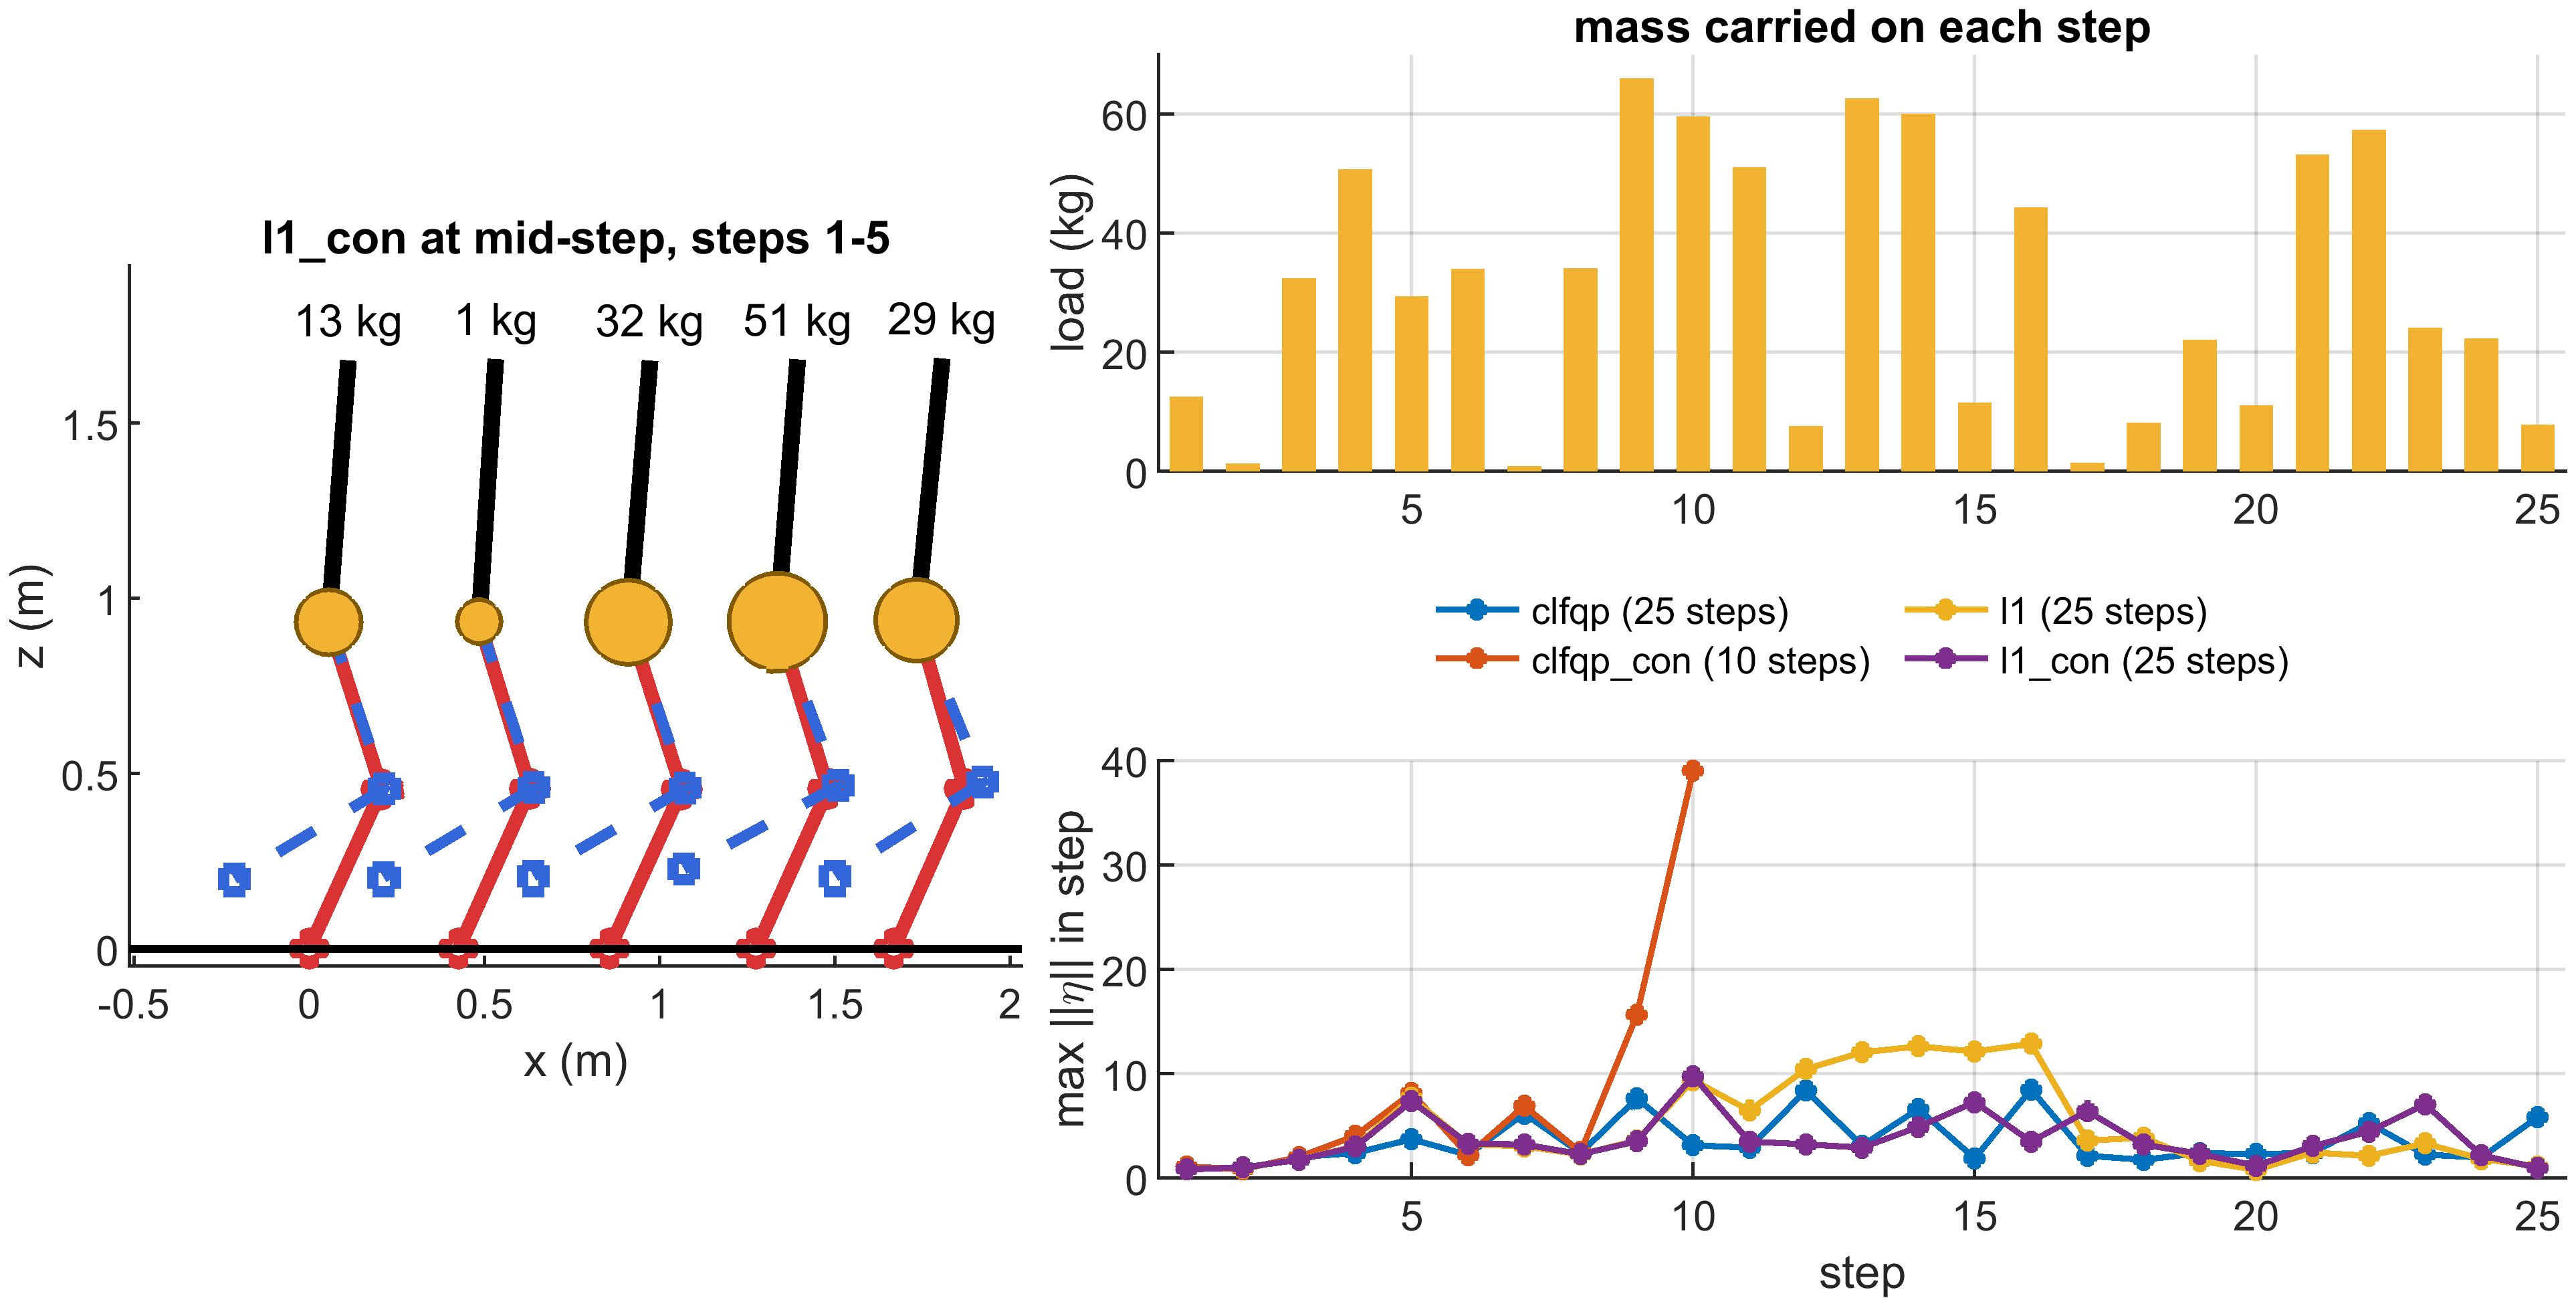
\includegraphics[width=\textwidth]{ch4_load_random.png}
    \caption{بازتولید شکل~\en{4.11}الف. سمت چپ: \code{l1\_con} در میانه گام‌های $1$ تا $5$،
    با اندازه دیسک ران متناسب با بار. بالا سمت راست: جرم حمل‌شده در هر گام. پایین سمت
    راست: بیشینه خطای ردیابی در هر گام. \code{clfqp\_con} پس از گام $10$ پایان
    می‌یابد؛ \code{l1} و \code{l1\_con} هر $25$ گام را طی می‌کنند، اما اعتبار
    فیزیکی \code{l1\_con} در گام $16$ و \code{l1} در گام $5$ از دست می‌رود.}
    \label{fig:loadrandom}
\end{figure*}

\textbf{بهای نرمال‌سازی درون همین $25$ گام} کوچک است: با جعبه یکسان، بدترین گام
\code{l1\_con} زیر بار تصادفی به $9.79$ می‌رسد و نیروی عمودی واقعی‌اش دست‌کم $3$
نیوتن می‌ماند. آنچه نرمال‌سازی می‌خرد در افق بلند است (جدول~\ref{tab:window}).

\begin{table*}[!t]
    \centering
    \caption{فراتر از سبک‌ترین بار، $\mathcal{L}_1$ بهتر از مبنای بدون قید ردیابی نمی‌کند
    (\code{clfqp} $|$ \code{l1\_con})}
    \label{tab:track}
    \small
    \begin{tabular}{lcccc}
        \toprule
        معیار & تصادفی & $23$ کیلوگرم & $35$ کیلوگرم & $46$ کیلوگرم \\
        \midrule
        گام نوعی: میانه بیشینه $\|\eta\|$ در هر گام & $5.29\;|\;3.51$ & $2.70\;|\;1.95$ & $2.64\;|\;5.09$ & $2.58\;|\;9.97$ \\
        بیشینه گشتاور (نیوتن‌متر) & $1922\;|\;556$ & $730\;|\;370$ & $1153\;|\;467$ & $1599\;|\;556$ \\
        گام‌های معتبر & $15\;|\;15$ & $2\;|\;25$ & $9\;|\;7$ & $6\;|\;2$ \\
        \bottomrule
    \end{tabular}
\end{table*}

جدول~\ref{tab:track} تصویر را کامل می‌کند. در $23$ کیلوگرم \code{l1\_con} هم گام
نوعی و هم بدترین گام را با حدود نیمی از گشتاور بیشینه بهتر ردیابی می‌کند، و تنها
آنجاست که هر $25$ گامش معتبر است. در $35$ و به‌ویژه $46$ کیلوگرم گام نوعی آن
\emph{بدتر} از مبنای بدون قید است ($5.09$ در برابر $2.64$ و $9.97$ در برابر
$2.58$) و اعتبارش نیز کمتر ($7$ در برابر $9$، و $2$ در برابر $6$ گام). زیر بار
تصادفی گام نوعی‌اش بهتر است و اعتبارش برابر. پس مزیت تطبیق با بار کاهش می‌یابد و
در سنگین‌ترین بار برمی‌گردد؛ آنچه \code{l1\_con} در همه حالت‌ها نگه می‌دارد، تنها
بودجه گشتاور است. مانند شکل~\en{4.11}ب، گشتاور $\mathcal{L}_1$ با بار رشد می‌کند و
هموار می‌ماند (شکل~\ref{fig:loadtorque}).

\begin{figure*}[t]
    \centering
    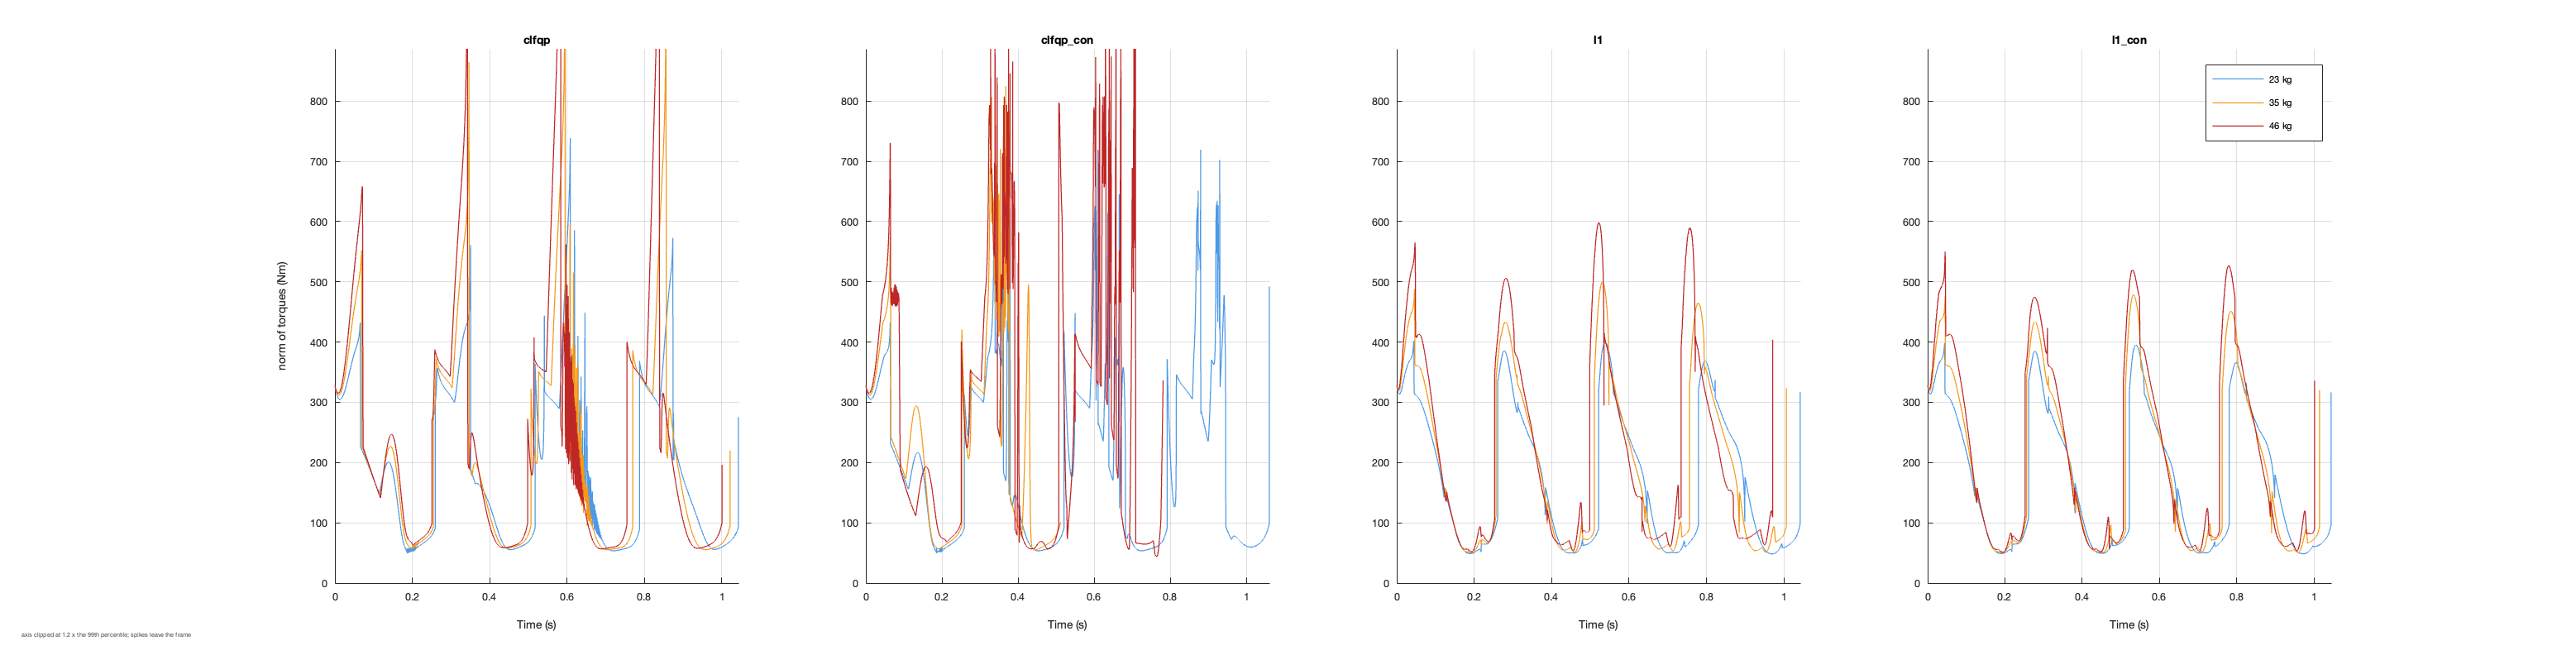
\includegraphics[width=\textwidth]{ch4_load_torque.png}
    \caption{بازتولید شکل~\en{4.11}ب: نرم گشتاورهای مفصل زیر بارهای $23$، $35$ و $46$
    کیلوگرم روی محوری مشترک. قله گام‌به‌گام \code{l1\_con} از $378$ به $476$ و $525$
    نیوتن‌متر می‌رسد؛ \en{CLF-QP} بدون قید در $35$ و $46$ کیلوگرم از $1000$ نیوتن‌متر
    فراتر می‌جهد و نسخه قیددار آن اشباع می‌شود و سقوط می‌کند.}
    \label{fig:loadtorque}
\end{figure*}

\begin{figure*}[t]
    \centering
    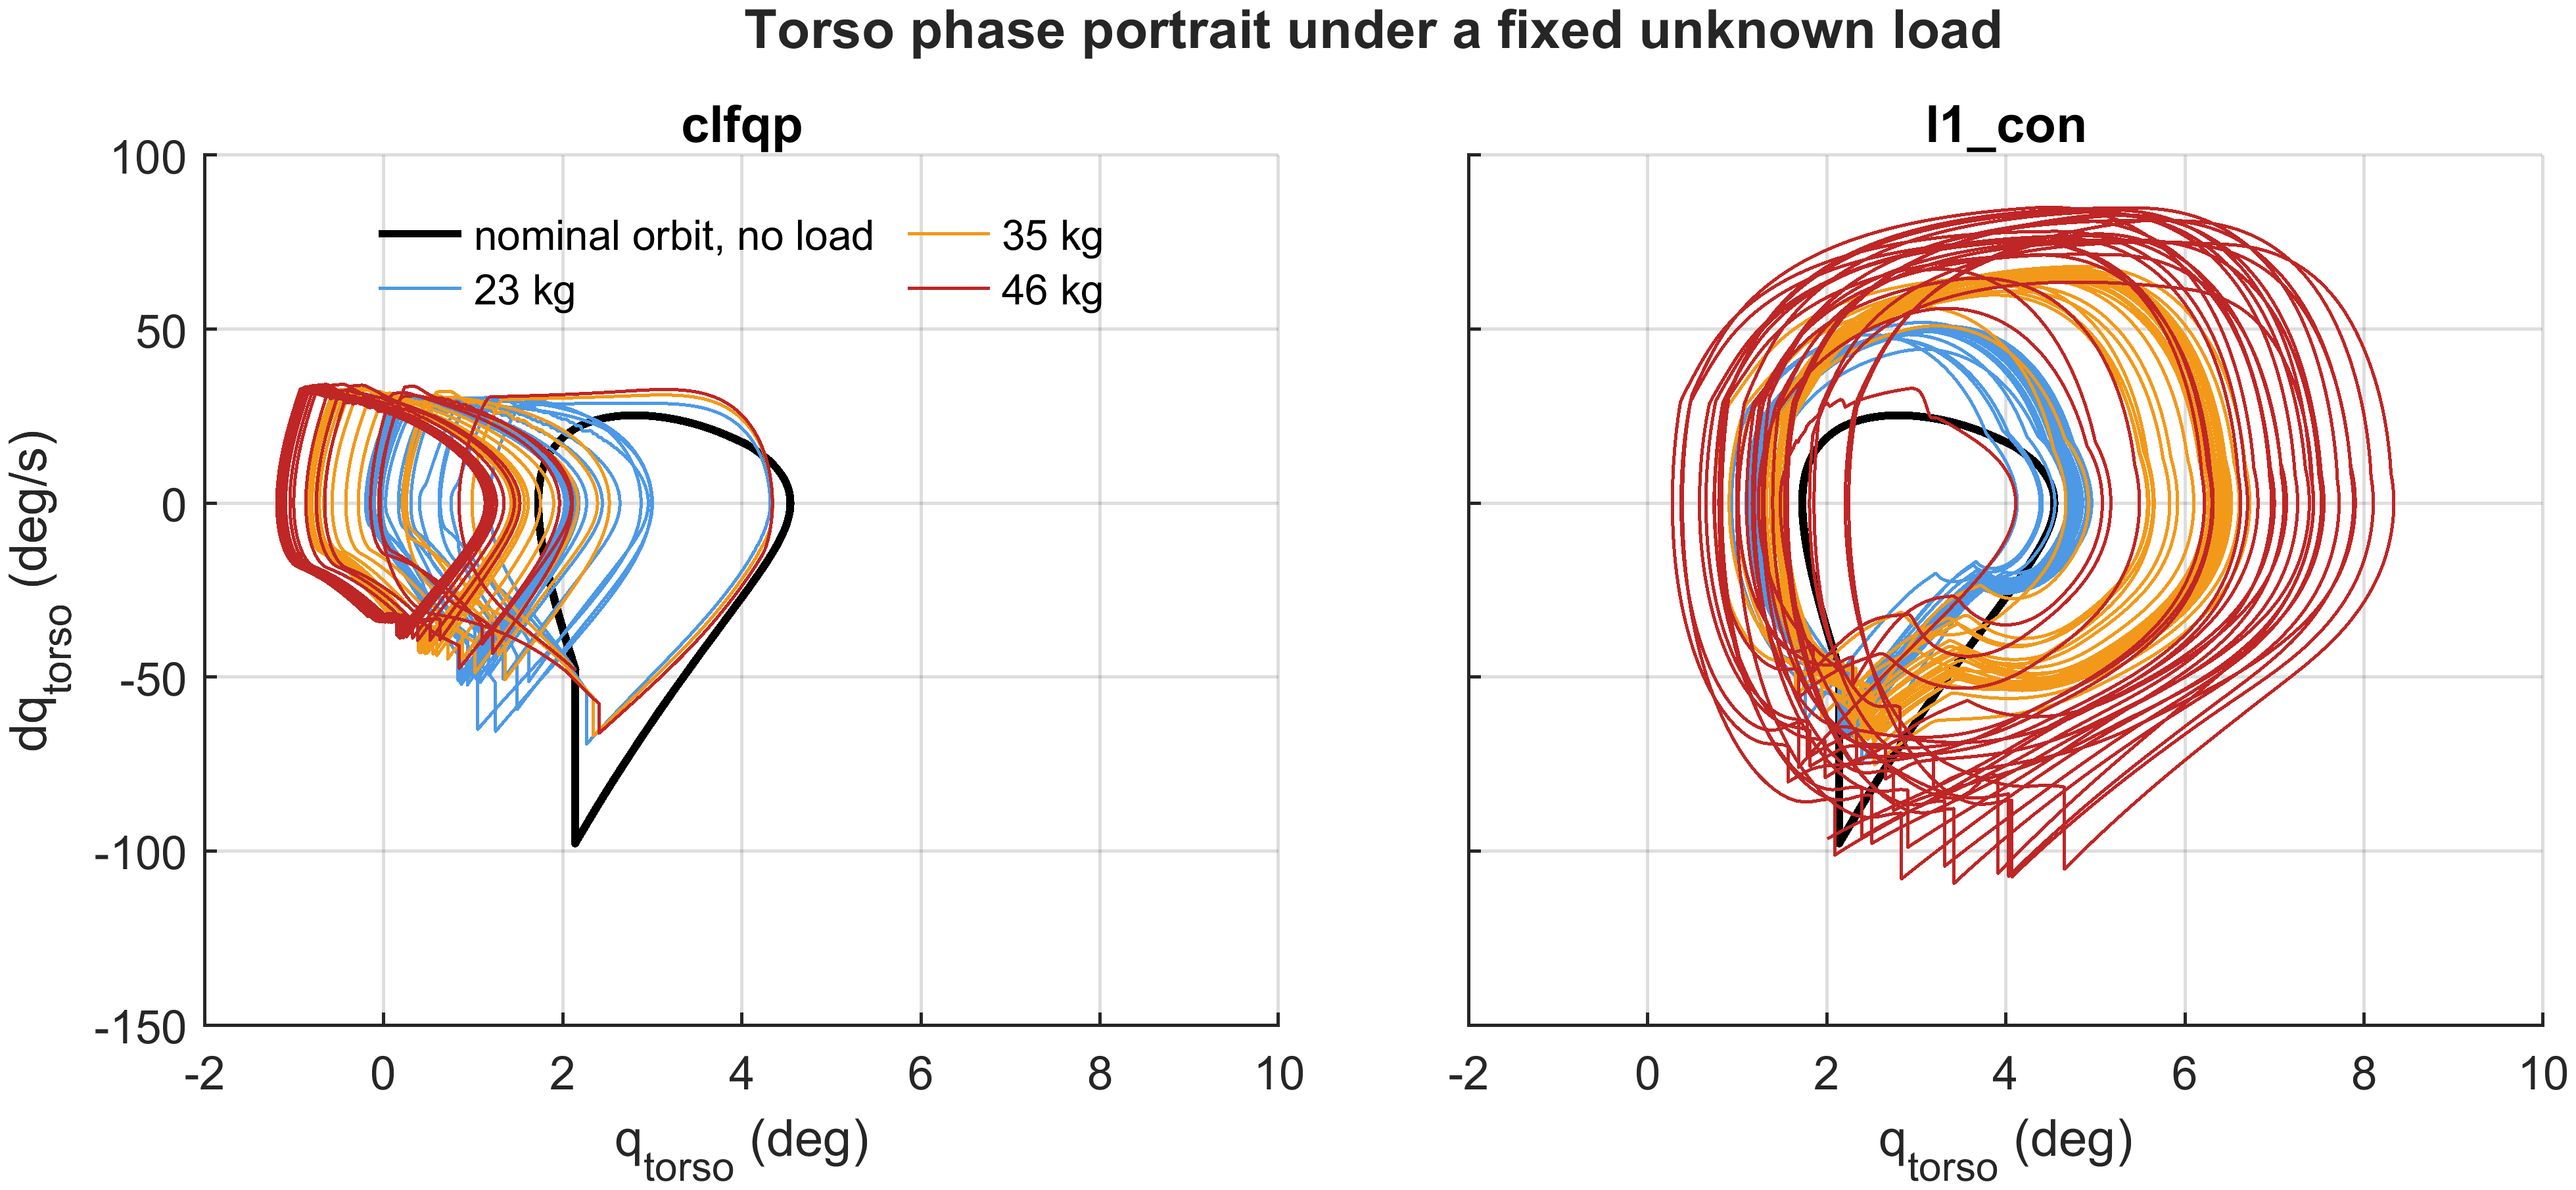
\includegraphics[width=\textwidth]{ch4_load_torso.png}
    \caption{تصویر فاز تنه زیر بار ثابت. مبنای بدون قید (چپ) $2$ تا $3$ درجه پایین‌تر از
    مدار اسمی می‌نشیند ($-1.2$ تا $2.1$ درجه در پنج گام آخر، در برابر $1.72$ تا $4.55$)،
    و چرخه \code{l1\_con} (راست) به $0.6$ تا $6.0$ درجه با نرخ گام تا $+68$ درجه بر
    ثانیه بزرگ می‌شود. بار، برخلاف مقیاس جرم، می‌تواند خودِ مدار را جابه‌جا کند؛ اما
    فاصله دو کنترل‌کننده زیر یک بار، خطای ردیابی است.}
    \label{fig:loadtorso}
\end{figure*}

% =====================================================================
\section{فراتر از افق متن مرجع}
\label{sec:long}
% =====================================================================
متن مرجع در $25$ گام متوقف می‌شود. با افزایش افق به $60$ گام ($120$ برای \code{l1} در
$\times1.5$) و تنها با سه اصلاح نخست، \code{l1\_con} در همه مقیاس‌های جرم پایدار ماند،
اما \code{l1} در $\times1.5$ در گام $76$ سقوط کرد، و زیر بار تصادفی \code{l1\_con} در
هر چهار دنباله آزموده\md{}گام‌های $43$، $33$، $55$ و $57$\md{}سقوط کرد، در حالی که
\en{CLF-QP} بدون قید هر $60$ گام همه آن‌ها را طی کرد.

\textbf{رانش واقعی است، اما نشانه است و نه علت.} پارامتربندی
$\hat\theta=\hat\alpha\|\eta\|+\hat\beta$ افزونه است: تا وقتی $\|\eta\|$ نزدیک یک مقدار
بماند، هر تقسیمی از $\theta$ میان $\hat\alpha$ و $\hat\beta$ پیش‌بینی یکسانی می‌دهد و
هیچ چیز این تقسیم را نگه نمی‌دارد. در اجراهای بلند دو تخمین به جهت‌های تقریباً مخالف
رانده می‌شوند (میانه کسینوس $-0.91$ در $\times0.7$ و $-0.95$ در $\times1.5$) و
$\hat\alpha$ به مرز تصویر خود فشار می‌آورد. نشت $\hat\alpha$ به سوی صفر وضع را بدتر کرد.

\textbf{سقوط‌ها از پیشی گرفتن حلقه تخمین‌گر بر نرخ نمونه‌برداری‌اند.} سه سقوط
نمونه‌به‌نمونه دوباره شبیه‌سازی شدند و هر سه چند میلی‌ثانیه پس از برخوردی آغاز
می‌شوند که $\|\eta\|$ را در $12$ تا $14$ رها می‌کند. در آنجا حلقه با حدود $4100$ رادیان
بر ثانیه کار می‌کند\md{}$4.1$ رادیان در هر نمونه، فراتر از حد پایداری حدوداً $2.8$
پیشروی رونگه-کوتا\md{}و ظرف $1$ تا $3$ نمونه $\hat\theta$ به $2700$ تا $2900$ می‌رسد، در
برابر $\theta$ واقعی $30$ تا $300$. گشتاور تطبیقی \en{QP} را از کار می‌اندازد و گام
فرو می‌ریزد. جدول~\ref{tab:mitig} آنچه آزموده شد را خلاصه می‌کند.

\begin{table*}[!t]
    \centering
    \caption{راه‌حل‌های آزموده روی نه اجرای بلند: \code{l1\_con} در $\times1$، $\times0.7$،
    $\times1.5$ و $46$ کیلوگرم ($60$ گام)، \code{l1} در $\times1.5$ ($120$ گام) و چهار
    دنباله بار تصادفی}
    \label{tab:mitig}
    \small
    \begin{tabular}{p{0.34\textwidth}cp{0.46\textwidth}}
        \toprule
        تغییر & سقوط از $9$ & اجرای تماماً معتبر از $9$ \\
        \midrule
        هیچ (تنها سه اصلاح نخست) & $4$ & $1$ \\
        نشت $\hat\alpha$ به سوی صفر با نرخ $2$ / $10$ / $50$ & $5$ / $5$ / $2$ & $1$ / $1$ / $\mathbf{5}$ \\
        پیوستگی $\hat\theta$ در برخورد پا / ادغام آن در $\hat\beta$ & $7$ / $6$ & $1$ / $1$ \\
        سقف رگرسور $\hat\alpha$، $1.5$ / $1$ / $0.5$ رادیان بر نمونه & $4$ / $3$ / $2$ & $1$ / $1$ / $2$ \\
        دوره کنترل $0.5$ میلی‌ثانیه، بدون تغییر دیگر ($6$ از $9$) & $0$ از $6$ & $1$ از $6$ \\
        تطبیق نرمال‌شده، صورت درسی (حلقه در $\sqrt\Gamma$) & $6$ & $1$ \\
        تطبیق نرمال‌شده، $\rho=0.5$ / $0.75$ / $1$ / $1.5$ / $2$ & $4$ / $\mathbf{1}$ / $3$ / $2$ / $1$ & $1$ / $2$ / $2$ / $1$ / $1$ \\
        \bottomrule
    \end{tabular}
\end{table*}

\textbf{نرمال‌سازی مانند یک پنجره عمل می‌کند} (جدول~\ref{tab:window}). در صورت درسی،
که حلقه را در هر خطایی در $\sqrt\Gamma$ نگه می‌دارد، تخمین‌گر زیر نرخ پیش‌بین
$a=800$ فرامیرا می‌شود و در راه‌رفتن عادی عقب می‌ماند. بالاتر از $\rho=1$ به‌ندرت فعال
می‌شود و سقوط‌ها در همان اجراهایی بازمی‌گردند که بدون آن سقوط می‌کردند. حدی که در
حلقه بسته اهمیت دارد، حدود $1$ رادیان بر نمونه، بسیار زیر حد $2.8$ خودِ پیشروی
رونگه-کوتاست؛ این تحلیل آن را اندازه می‌گیرد و استخراج نمی‌کند.

\begin{table}[H]
    \centering
    \caption{کسر اجراهای ساقط‌شده بر حسب سقف $\rho$ (رادیان بر نمونه): روی نه اجرایی
    که $\rho$ بر اساس آن‌ها انتخاب شد، و روی شش دنباله تازه}
    \label{tab:window}
    \small
    \begin{tabular}{lcc}
        \toprule
        $\rho$ & نه اجرای انتخاب & شش دنباله تازه \\
        \midrule
        $0.32$ (صورت درسی) & $6$ از $9$ & \nd{} \\
        $0.5$  & $4$ از $9$ & \nd{} \\
        $\mathbf{0.75}$ (انتخاب‌شده) & $\mathbf{1}$ از $9$ & $\mathbf{0}$ از $6$ \\
        $1$    & $3$ از $9$ & $3$ از $6$ \\
        $1.5$  & $2$ از $9$ & \nd{} \\
        $2$    & $1$ از $9$ & \nd{} \\
        بدون نرمال‌سازی & $4$ از $9$ & $4$ از $6$ \\
        \bottomrule
    \end{tabular}
\end{table}

از آنجا که $\rho$ روی همان نه اجرا انتخاب شد، گزینه‌ها روی شش دنباله تازه بار تصادفی
(\code{p.load\_seed} از $4$ تا $9$، \code{l1\_con}، $60$ گام) دوباره اجرا شدند
(جدول~\ref{tab:oos}).

\begin{table}[H]
    \centering
    \caption{خارج از نمونه: شش دنباله تازه بار تصادفی ($60$ گام). گام نوعی: میانه
    بیشینه $\|\eta\|$ در هر گام؛ بیشینه: بزرگ‌ترین $\|\eta\|$؛ معتبر: گام‌های معتبر
    در شش دنباله}
    \label{tab:oos}
    \footnotesize
    \begin{tabular}{lcccc}
        \toprule
        گونه & سقوط & گام نوعی & بیشینه & معتبر \\
        \midrule
        سه اصلاح نخست & $4$ & $2.95$ تا $3.63$ & $7.7$ تا $9.7$ & $2$ تا $26$ \\
        سقف رگرسور $0.5$ & $4$ & $4.16$ تا $6.98$ & $18.8$ تا $49.3$ & $2$ تا $9$ \\
        $\rho=0.75$ & $\mathbf{0}$ & $3.70$ تا $4.46$ & $9.8$ تا $67.6$ & $2$ تا $22$ \\
        $\rho=1$ & $3$ & $2.70$ تا $3.95$ & $7.6$ تا $40.0$ & $2$ تا $20$ \\
        دوره $0.5$ میلی‌ثانیه & $1$ & $3.08$ تا $3.63$ & $7.1$ تا $17.8$ & $3$ تا $\mathbf{60}$ \\
        \bottomrule
    \end{tabular}
\end{table}

در مجموع پانزده اجرای بلند، $\rho=0.75$ یک بار سقوط می‌کند، در برابر هشت بار بدون
نرمال‌سازی و شش بار با سقف رگرسور؛ روی شش دنباله تازه به‌تنهایی، هیچ سقوطی ندارد در
برابر چهار سقوط بدون نرمال‌سازی. این جمع نه اجرای انتخاب را با شش اجرای آزمون
درمی‌آمیزد.

\textbf{اما هیچ‌یک از این گونه‌ها اجرای $60$ گامیِ تماماً معتبری زیر بار تصادفی
نمی‌سازد.} در شش دنباله تازه، $\rho=0.75$ اعتبارش را میان گام‌های $2$ و $22$ از دست
می‌دهد و تنها دوره کنترل $0.5$ میلی‌ثانیه یک دنباله را تا گام $60$ معتبر می‌برد. پس
آنچه نرمال‌سازی می‌خرد، \emph{نیفتادن} است و نه راه‌رفتن فیزیکی بلندمدت؛ آنچه در این
افق واقعاً کمک می‌کند، نمونه‌برداری تندتر است. اجراهای کامل‌شده نیز همیشه تمیز
نیستند: سه دنباله تازه در $\rho=0.75$ از انحراف‌های $24$ تا $68$ می‌گذرند و باز راه
می‌روند. تنها حلقه تندتر هم ایمن است و هم
هموار: در $0.5$ میلی‌ثانیه، بدون هیچ حدی، قانون در دوازده اجرا یک بار سقوط کرد و روی
دنباله‌های تازه از $16$ فراتر نرفت.

\textbf{آنچه داده‌ها پشتیبانی می‌کنند، حلقه تندتر است.} روی شش دنباله تازه\md{}تنها
سنجه خارج از نمونه این بخش\md{}دوره $0.5$ میلی‌ثانیه بدون هیچ تنظیمی صفر سقوط دارد و
تنگ‌ترین پراکندگی را هم: بیشینه $16.0$ در برابر $49.8$ برای $\rho=0.75$. در برابر آن،
$\rho=0.75$ یک سقوط و $\rho=1$ دو سقوط دارد و این تفاوت، چنان‌که بالا آمد، از نظر
آماری قابل تمایز نیست؛ یعنی روی داده خارج از نمونه، نرمال‌سازی هیچ مقدار $\rho$
مشخصی را توجیه نمی‌کند. نتیجه‌ای که خودِ این اعداد می‌دهند این است:
\textbf{راه‌حل، نرخ نمونه‌برداری است و نرمال‌سازی وصله‌ای وابسته به نرخ است که در $1$
کیلوهرتز زمان می‌خرد.} هزینه آن دو برابر شدن زمان محاسبه در هر دوره است، که
بخش~\ref{sec:qptime} آن را اندازه می‌گیرد.

\textbf{گزینه انتخاب‌شده برای اعداد این گزارش: $\rho=0.75$ در $1$ کیلوهرتز}، زیرا
جدول‌های \ref{tab:l1} و \ref{tab:load} باید در نرخ متن مرجع با آن مقایسه شوند و نه
در نرخی که متن مرجع نمی‌شناسد. با آن، \code{l1} در $\times1.5$
هر $120$ گام را با خطای $2.0$ تا $2.9$ در هر ده گام طی می‌کند، \code{l1\_con} هر چهار
دنباله اصلی و پنج از شش دنباله تازه را کامل می‌کند و اجرای $46$ کیلوگرمی همچنان $60$
گام دوام می‌آورد. \code{l1\_con} در $\times1.5$ دیگر مانند پیش مستقر نمی‌شود: $4.8$ در
گام‌های $1$ تا $10$، $2.2$ تا $2.4$ تا گام $40$، و سپس $3.5$ و $5.5$. جدول‌های
\ref{tab:l1} و \ref{tab:load} با همین تنظیم دوباره اجرا شده‌اند.

% =====================================================================
\section{ملاحظات اندازه‌گیری‌شده}
% =====================================================================
\begin{table*}[!t]
    \centering
    \caption{ادعاهای فصل چهارم در برابر این پیاده‌سازی ($25$ گام، مگر آنکه ذکر شود)}
    \label{tab:claims}
    \small
    \begin{tabular}{p{0.32\textwidth}p{0.47\textwidth}c}
        \toprule
        ادعا & اندازه‌گیری‌شده & حکم \\
        \midrule
        همگرایی قانون مقاوم از اغتشاش اثر نمی‌پذیرد، در حالی که مبنا افت می‌کند (تذکر~\en{4.6}) &
            تقابل برقرار است\md{}$4.2$ و $4.3$ در برابر $14.5$ تا $16.6$\md{}اما خطای خودِ آن رشد
            می‌کند و با جعبه یکسان بزرگ‌ترین فلات ($9.1$) در حالت بدون اغتشاش است & تنها تقابل \\
        با مدل کامل قانون مقاوم بهتر از مبنا ردیابی می‌کند (تذکر~\en{4.7}) &
            تا گام $5$ درست است؛ سپس روی $\|\eta\|\approx9$ در برابر $0.25$ می‌نشیند & تنها در آغاز \\
        حالت \en{IV}: هر دو مبنا شکست می‌خورند، قانون مقاوم با افتی اندک راه می‌رود &
            \en{A} در گام $4$ و \en{B} در گام $3$ سقوط می‌کنند (هر دو $2$ گام معتبر)؛ \en{C}
            با $1.89$، هر $25$ گام معتبر، و $120$ گام معتبر در افق بلند & بازتولید شد \\
        راه‌رفتن حالت \en{IV} تا توقف کامل کند می‌شود &
            پس از $120$ گام $1.541$ متر بر ثانیه؛ دینامیک صفر ناوردا و پایدار است & بازتولید نشد \\
        بدون خطای مدل، $\mathcal{L}_1$ مانند \en{CLF-QP} عمل می‌کند &
            در زمان پیوسته دقیق؛ در $1$ کیلوهرتز خطای $0.14$ در برابر $0.25$ و $\|\hat\theta\|\le9$ & بازتولید شد \\
        همگرایی $\mathcal{L}_1$ از اغتشاش اثر نمی‌پذیرد (بخش~\en{4.2.4}) &
            با چهار اصلاح، گام‌ها در هر دو مقیاس کامل می‌شوند، اما تنها $\times1.5$ تماس معتبر
            دارد؛ در $\times0.7$ هیچ قانونی یک گام معتبر ندارد & تنها در $\times1.5$ \\
        $\mathcal{L}_1$ با بار ناشناخته تصادفی یا ثابت راه می‌رود (شکل~\en{4.11}) &
            گام‌ها در همه بارها کامل می‌شوند، اما تماس تنها در $23$ کیلوگرم برای هر $25$ گام
            معتبر است؛ در $35$ و $46$ کیلوگرم اعتبار به $7$ و $2$ گام می‌افتد & تنها در سبک‌ترین بار \\
        \bottomrule
    \end{tabular}
\end{table*}

\subsection{همه تضمین‌ها در زمان پیوسته‌اند؛ کنترل‌کننده نه}
هر دو راه‌حل به اصلاحی نیاز داشتند که تنها به دلیل نگهداری کنترل در یک دوره نمونه
وجود دارد: لایه مرزی، که همگرایی قانون مقاوم را به کران‌داری نهایی تبدیل می‌کند، و
نرمال‌سازی، که حلقه تخمین‌گر $\mathcal{L}_1$ را کندتر از نرخ نمونه‌برداری نگه
می‌دارد. حتی با مدل کامل، نگهداری ورودی در هر برخورد پا ضربه می‌زند
(جدول~\ref{tab:kick}): خطای پیش از برخورد در $1$ میلی‌ثانیه تنها
$6.8\times10^{-3}$ است و نگاشت برخورد آن را حدود $35$ برابر بزرگ می‌کند.

\begin{table}[H]
    \centering
    \caption{خطای ردیابی پس از نخستین برخورد پا با مدل کامل}
    \label{tab:kick}
    \small
    \begin{tabular}{lc}
        \toprule
        دوره کنترل & $\|\eta^+\|$ پس از گام $1$ \\
        \midrule
        $1$ میلی‌ثانیه (پیش‌فرض) & $0.242$ \\
        $0.5$ میلی‌ثانیه & $0.123$ \\
        $0.2$ میلی‌ثانیه & $0.049$ \\
        پیوسته & $1.7\times10^{-4}$ \\
        \bottomrule
    \end{tabular}
\end{table}

\subsection{تذکر~\en{4.4}، اندازه‌گیری‌شده}
قیدهای اصطکاک، پیش‌بینی \emph{اسمی} را در $\mu\le0.4$ نگه می‌دارند. در $25$ گام، صدک
نود و پنجم تقاضای واقعی در حالت‌های \en{I} تا \en{III} برابر $0.22$، $0.12$ و $0.26$
است، با قله‌های $0.25$ و $0.39$ در حالت‌های \en{I} و \en{II}؛ و در $\times0.7$ لحظه‌ای
به $1.49$ می‌رسد: لغزشی گذرا که کنترل‌کننده نمی‌تواند ببیند، و درست همان شکافی که
تذکر~\en{4.4} درباره آن هشدار می‌دهد. نیروهای تماس در این گزارش همواره از مدل واقعی
محاسبه شده‌اند؛ اگر از مدل خودِ کنترل‌کننده محاسبه می‌شدند، در $\times1.5$ پنجاه درصد
خطا داشتند.

\subsection{هزینه محاسباتی یک ارزیابی کنترل}
\label{sec:qptime}
نتیجه مرکزی این فصل آن است که اثرهای نمونه‌برداری‌شده غالب‌اند و تمیزترین راه‌حلِ
اندازه‌گیری‌شده، دوره کنترل کوتاه‌تر است. این توصیه تنها وقتی معنا دارد که حلقه در آن
نرخ بسته شود، پس باید گفت یک ارزیابی چقدر هزینه دارد. جدول~\ref{tab:qptime} این را
اندازه می‌گیرد: یک فراخوانی \code{ch4\_control}، یعنی حل برنامه درجه دوم به‌همراه
خطی‌سازی ورودی\nd{}خروجی پیرامون آن، روی $200$ حالت \emph{در طول} یک گام از مدار
مرجع و با $25$ تکرار در هر حالت، در مقیاس $\times1.5$ تا سطرهای قیددار واقعاً فشار
بیاورند.

\begin{table}[H]
    \centering
    \caption{زمان دیواری یک ارزیابی کنترل (میکروثانیه)، $200$ حالت در طول یک گام،
    مقیاس $\times1.5$}
    \label{tab:qptime}
    \small
    \begin{tabular}{lcccc}
        \toprule
        قانون & میانه & $p_{90}$ & $p_{99}$ & بیشینه \\
        \midrule
        \code{clfqp}      & $83.8$  & $101.0$ & $153.4$  & $231.9$ \\
        \code{clfqp\_con}  & $293.1$ & $349.9$ & $445.6$  & $3019.1$ \\
        \code{rclfqp\_con} & $367.5$ & $603.2$ & $1105.6$ & $3302.1$ \\
        \code{l1}         & $186.5$ & $220.8$ & $256.6$  & $1213.6$ \\
        \code{l1\_con}     & $322.2$ & $428.9$ & $691.3$  & $837.5$ \\
        \bottomrule
    \end{tabular}
\end{table}

\textbf{این اعداد را باید با احتیاط خواند.} اینجا \en{MATLAB} مفسری است که
\code{quadprog} را روی یک رایانه رومیزی صدا می‌زند؛ این یک کران بالا برای یک
پیاده‌سازی کامپایل‌شده است، با فاصله‌ای زیاد و اندازه‌گیری‌نشده، و \emph{ادعایی درباره
شدنی‌بودن روی سخت‌افزار نهفته نیست}. آنچه معتبرتر است نسبت‌هاست، که به پیاده‌سازی
بسیار کمتر وابسته‌اند.

با همین قید، سه چیز خوانده می‌شود. نخست، \textbf{قید هزینه دارد}: افزودن جعبه و
سطرهای تماس میانه را از $84$ به $293$ میکروثانیه می‌برد، یعنی $3.5$ برابر، و جمله
مقاوم آن را به $368$ می‌رساند. دوم، در میانه هیچ قانونی به بودجه $1000$
میکروثانیه‌ای نزدیک نمی‌شود و حتی بودجه $500$ میکروثانیه‌ای حلقه $2$ کیلوهرتزی نیز
برای هر پنج قانون در میانه و در $p_{90}$ برقرار است\md{}جز \code{rclfqp\_con} که
$p_{90}$ آن $603$ است. سوم و مهم‌تر از همه، \textbf{دنباله است که بودجه را می‌شکند
و نه میانه}: بیشینه \code{clfqp\_con} و \code{rclfqp\_con} به $3019$ و $3302$
میکروثانیه می‌رسد، یعنی سه برابر یک دوره $1$ کیلوهرتزی. این قله‌ها در حالت‌های پس از
برخورد رخ می‌دهند، جایی که $\|\eta\|$ بزرگ است و سطرها با هم در تعارض‌اند\md{}دقیقاً
همان‌جا که فصل نشان داد حلقه تخمین‌گر از نرخ نمونه‌برداری پیشی می‌گیرد.

پس توصیه دوره $0.5$ میلی‌ثانیه رایگان نیست، اما در این محیط هم غیرممکن نیست: برای
\code{l1\_con}، که قانون توصیه‌شده این فصل است، $p_{99}$ برابر $691$ میکروثانیه و
بیشینه $838$ میکروثانیه است، یعنی $1.4$ و $1.7$ برابر یک دوره $0.5$ میلی‌ثانیه‌ای.
یک پیاده‌سازی کامپایل‌شده با ضریب چندبرابری که معمول است این فاصله را می‌پوشاند، اما
این گزارش آن ضریب را اندازه نگرفته است و آن را ادعا نمی‌کند.

\subsection{جعبه‌های گشتاور از حد عملگر اعلام‌شده بسیار فراترند}
\label{sec:budget}
حد گشتاور اعلام‌شده این ربات $120$ نیوتن‌متر است (فصل سوم، \code{ch3\_params}). این
فصل اکنون یک مشخصه عملگر \emph{واحد} به کار می‌برد\md{}$556$ نیوتن‌متر برای همه
کنترل‌کننده‌ها، همه مقیاس‌های جرم و همه بارها، و $731$ نیوتن‌متر برای حالت \en{IV} که
بیرون از پوش طراحی است\md{}که مسئله جعبه‌های ساخته‌شده از اغتشاشِ پیشِ رو را برطرف
می‌کند. اما مسئله دیگری را برطرف نمی‌کند: $556$ و $731$ به ترتیب $4.6$ و $6.1$ برابر
حد اعلام‌شده‌اند.

نتیجه را باید صریح گفت: \textbf{بخش مقیاس جرم این فصل یک مطالعه جبری است و نه یک
مطالعه شدنی‌بودن.} گزاره «قانون مقاوم جایی راه می‌رود که مبناها سقوط می‌کنند» گزاره‌ای
درباره رباتی است که با عملگرهای اعلام‌شده خود ساخته نمی‌شود. آنچه این بخش نشان می‌دهد
معتبر است\md{}ترتیب نسبی سه قانون، ساختار $\Delta_1$ و $\Delta_2$، و رفتار لایه
مرزی\md{}اما هیچ‌یک از اعداد گام را نباید ادعای عملکردِ سخت‌افزاری خواند. مقایسه در
بودجه گشتاور واقعی $120$ نیوتن‌متری در بخش~\ref{sec:box120} انجام شده است.


\subsection{مقایسه در بودجه $120$ نیوتن‌متری}
\label{sec:box120}
این مقایسه اکنون انجام شده است. هر پنج کنترل‌کننده فصل، با \emph{یک} جعبه $120$
نیوتن‌متری\md{}حد اعلام‌شده خودِ ربات\md{}و بدون هیچ تغییر دیگری، روی همان گام
\code{posture\_195} و در $25$ گام اجرا شدند (جدول~\ref{tab:box120}).

\begin{table*}[!t]
    \centering
    \caption{همان کنترل‌کننده‌ها زیر جعبه $120$ نیوتن‌متری، حد عملگر اعلام‌شده ربات،
    در $25$ گام. هر خانه: تعداد گام $|$ گام‌های معتبر $|$ بیشینه گشتاور کشیده‌شده
    (نیوتن‌متر). خط تیره یعنی حتی یک گام کامل نشد. سطرهای پررنگ آن‌هایی‌اند که جعبه،
    گشتاور \emph{اعمال‌شده}‌شان را مقید می‌کند}
    \label{tab:box120}
    \small
    \begin{tabular}{lccc}
        \toprule
        کنترل‌کننده & $\times1$ (مدل کامل) & $\times1.5$ & $\times0.7$ \\
        \midrule
        \code{clfqp} (بی‌جعبه)          & $25\;|\;1\;|\;198$ & $25\;|\;0\;|\;1372$ & $25\;|\;0\;|\;524$ \\
        \code{l1} (جعبه فقط روی $\mu_1$) & $25\;|\;25\;|\;197$ & $25\;|\;0\;|\;396$ & $25\;|\;0\;|\;335$ \\
        \midrule
        \textbf{\code{clfqp\_con}}   & $\mathbf{1\;|\;0\;|\;120}$ & \nd{} & $\mathbf{1\;|\;0\;|\;120}$ \\
        \textbf{\code{rclfqp\_con}}  & \nd{} & \nd{} & $\mathbf{1\;|\;0\;|\;120}$ \\
        \textbf{\code{l1\_con}}      & $\mathbf{1\;|\;0\;|\;120}$ & \nd{} & $\mathbf{3\;|\;1\;|\;120}$ \\
        \bottomrule
    \end{tabular}
\end{table*}

\textbf{نتیجه یک‌دست است.} هر قانونی که جعبه، گشتاور \emph{اعمال‌شده} آن را مقید
می‌کند\md{}سه سطر پایین جدول\md{}در $120$ نیوتن‌متر در فاصله صفر تا سه گام از پا
درمی‌آید، و این شامل $\times1$ یعنی \textbf{مدل کامل} هم می‌شود: قانون مقاوم در
$\times1$ حتی یک گام کامل ندارد و در نخستین گام تنها $0.014$ متر جابه‌جا می‌شود.
در هیچ خانه‌ای از این سه سطر بیش از یک گام \emph{معتبر} وجود ندارد.

\textbf{و آن‌ها که راه می‌روند، از جعبه بیرون‌اند.} دو سطر بالای جدول هر $25$ گام را
کامل می‌کنند، اما با کشیدن $197$ تا $1372$ نیوتن‌متر، یعنی دقیقاً به این دلیل که جعبه
$120$ نیوتن‌متری بر گشتاور اعمال‌شده آن‌ها نمی‌نشیند: \code{clfqp} اصلاً جعبه‌ای ندارد،
و \code{l1} در صورت متن مرجع تنها $\mu_1$ را در جعبه می‌گذارد، پس $\mu_2$ بیرون از هر
قیدی به مفاصل می‌رسد (اصلاح~$3$ بخش کنترل تطبیقی). تنها اجرای سراسر معتبر کل جدول،
\code{l1} در $\times1$ با $25$ گام معتبر است\md{}که $196.7$ نیوتن‌متر می‌کشد،
$1.64$ برابر حدی که قرار بود رعایت کند.

\textbf{شیوه از پا درآمدن، خودش تشخیص است.} هیچ‌یک از این سقوط‌ها لغزش یا بلندشدن پا
نیست؛ ربات یا \emph{به عقب} گام برمی‌دارد ($-0.084$ تا $-0.119$ متر) یا لگنش تا
$0.17$ متر فرومی‌افتد. این سیمای یک ربات گشتاورگرسنه است: نه می‌تواند پای نوسانی را
جلو بیندازد و نه می‌تواند خودش را بالا نگه دارد.

\textbf{و علت، بالادست این فصل است.} پیش‌خور خودِ گام مرجع به $195$ نیوتن‌متر
می‌رسد، یعنی $1.63$ برابر حد $120$ نیوتن‌متری، \emph{پیش از} آنکه هیچ اغتشاشی،
هیچ کنترل‌کننده‌ای و هیچ تطبیقی وارد شود. در $120$ نیوتن‌متر هیچ قانونی نمی‌تواند این
گام را ردیابی کند، چون گشتاور لازم برای ردیابی آن از بودجه بیشتر است. بنابراین این
مقایسه \textbf{سه قانون را از هم جدا نمی‌کند}؛ آنچه می‌سنجد گام است و نه
کنترل‌کننده‌ها.

این پاسخ، گزاره فصل را دقیق‌تر می‌کند و آن را پس نمی‌گیرد: نتایج $556$ نیوتن‌متری
همچنان ترتیب نسبی سه قانون را نشان می‌دهند، اما اکنون می‌دانیم که در بودجه واقعی
عملگر، هیچ‌کدام از آن‌ها روی \emph{این} گام راه نمی‌رود. کار باقی‌مانده از فصل چهارم
به فصل سوم منتقل می‌شود: گامی که زیر جعبه $120$ نیوتن‌متری بهینه شده باشد، و آنگاه
همین جدول دوباره معنا پیدا می‌کند. داده‌های این بخش در \code{Results/box120/}
ذخیره شده‌اند.

\subsection{نتایج $\times1.5$ حاصل تنظیم‌اند، نه حاشیه}
جاروب نرخ پیش‌بین، پنجره $\rho$ با لبه‌هایی در $0.5$ و $1.5$ که هر کدام دو سقوط از نه
دارند، و دنباله‌ای منفرد که هر حد $1$ کیلوهرتزی را شکست می‌دهد، همه یک چیز می‌گویند:
در مقیاس $\times1.5$ و زیر باری که هر گام از نو کشیده می‌شود، $\mathcal{L}_1$ در
$1$ کیلوهرتز همان‌جا کار می‌کند که برایش تنظیم شده است. جاروب‌ها گزارش شده‌اند تا این
ادعا سنجیدنی باشد و نه پذیرفتنی.

% =====================================================================
\section{اعتبارسنجی نرم‌افزاری}
% =====================================================================
مجموعه آزمون در سه لایه سازمان یافته و ترتیب آن ترتیب اشکال‌زدایی است: ابتدا تفکیک
مدل، سپس جبر هر کنترل‌کننده، و در پایان رفتاری که فصل ادعا می‌کند
(جدول~\ref{tab:tests}).

\begin{table}[H]
    \centering
    \caption{مجموعه آزمون فصل چهارم: $50$ بررسی، بدون خطا، در $9.8$ ثانیه}
    \label{tab:tests}
    \small
    \begin{tabular}{lcc}
        \toprule
        پیمانه & تعداد بررسی & نتیجه \\
        \midrule
        تفکیک مدل، ساختار $\Delta$ و بار & $17$ & قبول \\
        قانون مقاوم و لایه مرزی & $14$ & قبول \\
        کنترل $\mathcal{L}_1$ & $19$ & قبول \\
        \midrule
        \textbf{مجموع} & $\mathbf{50}$ & \textbf{قبول} \\
        \bottomrule
    \end{tabular}
\end{table}

دو بررسی به‌ویژه شایان ذکرند، زیرا در برابر \emph{نادرستی خاموش} محافظت می‌کنند.
نخست، تصدیق اینکه قانون فصل سوم شرط مقاوم را روی $294$ از $1200$ عدم قطعیت نمونه‌برداری‌شده
نقض می‌کند؛ بدون آن، آزمون‌های مقاوم می‌توانستند به‌طور بدیهی قبول شوند. دوم، دو
این همانی که فصل چهارم را به فصل سوم پیوند می‌دهند: با $D_1=D_2=0$ قانون مقاوم
\emph{همان} \en{CLF-QP} است ($3.4\times10^{-13}$)، و بدون خطای مدل $\mathcal{L}_1$
هیچ چیز را تطبیق نمی‌دهد، با خطای صفر. آزمون حلقه تخمین‌گر در $\|\eta\|=13$ نیز
واگرایی قانون بدون نرمال‌سازی و استقرار قانون نرمال‌شده را جداگانه تصدیق می‌کند.

% =====================================================================
\section{نتیجه‌گیری}
% =====================================================================
جدول~\ref{tab:claims} ادعاهای فصل چهارم را در برابر این پیاده‌سازی می‌سنجد. قانون
مقاوم در هر چهار مقیاس جرم راه می‌رود و حالت \en{IV} را، جایی که هر دو مبنا سقوط
می‌کنند، پشت سر می‌گذارد؛ اما خطای خودِ آن با اغتشاش رشد می‌کند و مزیت آن با مدل کامل
تنها در گام‌های نخست پابرجاست. کنترل $\mathcal{L}_1$ ادعای خود را تنها پس از چهار اصلاح
بازتولید می‌کند، و آنگاه زیر بار ناشناخته جایی راه می‌رود که \en{CLF-QP} با همان
بودجه گشتاور نمی‌تواند\md{}هرچند در سه حالت از چهار حالت بار، نیروی عمودی واقعی آن
منفی می‌شود و آن اجراها به تعریف خودِ این گزارش راه‌رفتن فیزیکی معتبری نیستند.

\textbf{دو هشدار پیش از هر چیز دیگر.} نخست، \textbf{همه این نتایج پیش‌گویانه‌اند}:
کران‌های $D_1=279.1$ و $D_2=0.514$ از خودِ اغتشاش اندازه‌گیری شده‌اند و در عمل در
اختیار کنترل‌کننده نیستند. جعبه گشتاور دیگر چنین نیست\md{}یک مشخصه واحد $556$
نیوتن‌متری برای همه حالت‌ها به کار می‌رود و از حالتی که اجرا می‌شود ساخته نمی‌شود\md{}
پس هشدار پیش‌گویی اکنون تنها به $D_1$ و $D_2$ مربوط است و نه به بودجه گشتاور.
جمله «قانون مقاوم در هر چهار مقیاس جرم راه می‌رود» را باید با همین قید خواند: راه
می‌رود، به شرط آنکه کسی اندازه اغتشاش را از پیش به او گفته باشد. دوم،
\textbf{مشخصه عملگر این فصل، $556$ نیوتن‌متر (و $731$ در حالت \en{IV})، به ترتیب
$4.6$ و $6.1$ برابر حد اعلام‌شده $120$ نیوتن‌متری این ربات است}
(بخش~\ref{sec:budget})، پس بخش مقیاس جرم یک مطالعه جبری است و نه مطالعه
شدنی‌بودن؛ ترتیب نسبی سه قانون معتبر می‌ماند، اما هیچ عدد گامی ادعای عملکرد
سخت‌افزاری نیست. این مقایسه اکنون در بودجه واقعی $120$ نیوتن‌متری انجام شده است
(بخش~\ref{sec:box120}): هیچ‌یک از سه قانونی که جعبه، گشتاور اعمال‌شده‌شان را مقید
می‌کند بیش از سه گام دوام نمی‌آورد، و این شامل $\times1$ با مدل کامل هم می‌شود. چون
پیش‌خور خودِ گام مرجع $1.63$ برابر آن حد است، این یافته گزاره‌ای درباره \emph{گام}
است و نه درباره کنترل‌کننده‌ها؛ کار باقی‌مانده، گامی است که زیر جعبه $120$
نیوتن‌متری بهینه شده باشد.


چند محدودیت باید همراه این نتایج حمل شوند. نخست، \textbf{قیدهای تماس تنها به اندازه
مدل خوب‌اند}: هر سطر اصطکاک و نیروی عمودی یک پیش‌بینی را مقید می‌کند و تقاضای واقعی
اصطکاک به $1.49$ در برابر سطری با $0.4$ رسید؛ متن مرجع در فصل هشتم به قیدهای تماس
بازمی‌گردد و فصل چهارم آن‌ها را مقاوم نمی‌کند. دوم، \textbf{کران مقاوم نمی‌تواند باری
واقعی را پوشش دهد}: برای بار روی ران $\|\Delta_2\|$ میان $2.0$ و $2.7$ است، بیرون از هر
کرانی که قانون مقاوم بتواند به کار گیرد، و حتی درون کران، قانون با مدل کامل خطای پایا
می‌پردازد. سوم، \textbf{$\mathcal{L}_1$ در $1$ کیلوهرتز به طراحی آگاه از نرخ
نمونه‌برداری نیاز دارد} و همچنان در یک از شش دنباله تازه سقوط می‌کند؛ $\rho$
انتخاب‌شده در پنجره‌ای قرار دارد که روی همین ربات اندازه‌گیری شده است، و هر جا سخت‌افزار
اجازه دهد، حلقه تندتر راه‌حل تمیزتری است. سرانجام، \textbf{توابع سد فصل پنجم نیز
مبتنی بر مدل‌اند}؛ ترکیب یک سد نمایی مقاوم یا تطبیقی، گام طبیعی پیوند این دو فصل است
که هیچ‌کدام آن را نمی‌آزماید \cite{nguyen2016ecbf,xu2015robustness}.

% ---------------------- مراجع ----------------------
\begin{LTR}
\printbibliography[title={مراجع}]
\end{LTR}


% =====================================================================
% پیوست: استخراج روابط
% =====================================================================
\onecolumn
\setcounter{section}{0}
\renewcommand{\thesection}{پ}
\renewcommand{\thesubsection}{پ-\arabic{subsection}}
\section{استخراج روابط}
\label{app:deriv}
این پیوست هر رابطه متن را گام‌به‌گام از رابطه پیش از خود به دست می‌آورد و ترتیب آن
همان ترتیب متن است. نمادگذاری: $\eta=(y,\dot y)$ خطای ردیابی،
$V=\eta^{\mathsf T}P\eta$ تابع لیاپانوف فصل سوم، و
$\dot\eta=F\eta+G\mu$ با $G=\begin{bmatrix}0\\ I\end{bmatrix}$. علامت مد
($\tilde f,\tilde g$) مدل \textbf{اسمی} است که کنترل‌کننده در اختیار دارد و بدون
مد، ربات \textbf{واقعی}. برای اختصار $A:=L_gL_fy$ و $\tilde A:=L_{\tilde g}L_{\tilde f}y$.

% ---------------------------------------------------------------------
\subsection{منشأ $\Delta_1$ و $\Delta_2$ (روابط~\eqref{eq:unc} و \eqref{eq:deltas})}
دینامیک خروجی ربات واقعی $\ddot y=L_f^2y+A\,u$ است. کنترل‌کننده $u$ را از مدل اسمی
می‌سازد: پیش‌خور، رانش اسمی را خنثی می‌کند، $\tilde u_{\mathrm{ff}}=-\tilde A^{-1}L_{\tilde f}^2y$، پس
\begin{equation*}
    u=-\tilde A^{-1}L_{\tilde f}^2y+\tilde A^{-1}\mu .
\end{equation*}
با جای‌گذاری در دینامیک واقعی و افزودن و کاستن $\mu$:
\begin{equation*}
    \ddot y=L_f^2y-A\tilde A^{-1}L_{\tilde f}^2y+A\tilde A^{-1}\mu
    =\mu+\underbrace{\big(L_f^2y-A\tilde A^{-1}L_{\tilde f}^2y\big)}_{\Delta_1}
    +\underbrace{\big(A\tilde A^{-1}-I\big)}_{\Delta_2}\mu .
\end{equation*}
اگر مدل دقیق باشد ($A=\tilde A$ و $L_f^2y=L_{\tilde f}^2y$) هر دو جمله صفر می‌شوند و
$\ddot y=\mu$ فصل سوم بازمی‌گردد.

% ---------------------------------------------------------------------
\subsection{مقیاس یکنواخت جرم (رابطه~\eqref{eq:scale})}
در فاز اتکا، دینامیک همراه با قید تماس یک دستگاه \en{KKT} است:
\begin{equation*}
    \begin{bmatrix}D & J^{\mathsf T}\\ J & 0\end{bmatrix}
    \begin{bmatrix}\ddot q\\ \lambda\end{bmatrix}
    =\begin{bmatrix}-C\dot q-G_{\mathrm{grav}}+Bu\\ -\dot J\dot q\end{bmatrix}.
\end{equation*}
مقیاس جرم و اینرسی با $s$ یعنی $D\to sD$، $C\to sC$ و
$G_{\mathrm{grav}}\to sG_{\mathrm{grav}}$؛ ژاکوبین تماس $J$ هندسی است و تغییر نمی‌کند.
با تقسیم سطر بالا بر $s$ و در نظر گرفتن $\lambda/s$ به‌عنوان مجهول:
\begin{equation*}
    \begin{bmatrix}D & J^{\mathsf T}\\ J & 0\end{bmatrix}
    \begin{bmatrix}\ddot q\\ \lambda/s\end{bmatrix}
    =\begin{bmatrix}-C\dot q-G_{\mathrm{grav}}+\tfrac1s Bu\\ -\dot J\dot q\end{bmatrix}.
\end{equation*}
این همان دستگاه اسمی است که در آن $u$ با $u/s$ جایگزین شده. بنابراین شتاب رانش مستقل
از $s$ است، $L_f^2y=L_{\tilde f}^2y$، و شتاب ورودی با $1/s$ مقیاس می‌گیرد،
$A=\tfrac1s\tilde A$. جای‌گذاری در بخش قبل:
\begin{equation*}
    \Delta_2=\tfrac1s\tilde A\tilde A^{-1}-I=\Big(\tfrac1s-1\Big)I,\qquad
    \Delta_1=L_{\tilde f}^2y-\tfrac1s L_{\tilde f}^2y=-\Big(\tfrac1s-1\Big)L_{\tilde f}^2y .
\end{equation*}
سه نتیجه: (۱)~$\|\Delta_2\|<1\iff|1/s-1|<1\iff 0<1/s<2\iff s>0.5$.
(۲)~همان حرکت به $u\to s\,u$ نیاز دارد؛ پس جعبه گشتاور باید تا $s$ برابر پیش‌خور را
بردارد و رده $556$ نیوتن‌متری از $195\times1.5=293$ نیوتن‌متر فراتر است.
(۳)~باری که به ران آویخته شود $D$ را غیریکنواخت تغییر می‌دهد (نه به صورت $sD$)،
دستگاه جدا نمی‌شود و $\Delta_2$ دیگر مضربی از $I$ نیست.

% ---------------------------------------------------------------------
\subsection{مشتق $V$ تحت عدم قطعیت}
با عدم قطعیت، $\dot\eta=F\eta+G(\mu+\Delta_1+\Delta_2\mu)$، پس
\begin{equation*}
    \dot V=\eta^{\mathsf T}(F^{\mathsf T}P+PF)\eta+2\eta^{\mathsf T}PG\,(\mu+\Delta_1+\Delta_2\mu)
    =L_fV+L_gV\,\Delta_1+L_gV\,(I+\Delta_2)\,\mu ,
\end{equation*}
با همان تعاریف فصل سوم: $L_fV=\eta^{\mathsf T}(F^{\mathsf T}P+PF)\eta$ و
$L_gV=2\eta^{\mathsf T}PG$.

% ---------------------------------------------------------------------
\subsection{قانون مقاوم $\mu^*$ (رابطه~\eqref{eq:rclf})}
شرط $\dot V\le-(c_3/\varepsilon)V$ باید برای \emph{هر} عدم قطعیت مجاز برقرار باشد. با
$\psi=L_fV+(c_3/\varepsilon)V$:
\begin{equation*}
    \max_{\|\Delta_1\|\le D_1,\ |d_2|\le D_2}\ \psi+L_gV\,\Delta_1+L_gV\,\mu+d_2\,L_gV\,\mu\ \le 0 .
\end{equation*}

\textbf{گام ۱: جمله $\Delta_1$.} طبق نامساوی کوشی\nd{}شوارتز،
$L_gV\,\Delta_1\le\|L_gV\|\,\|\Delta_1\|\le D_1\|L_gV\|$، و تساوی در
$\Delta_1=D_1L_gV^{\mathsf T}/\|L_gV\|$ رخ می‌دهد. این بدترین حالت به $\mu$ وابسته نیست،
پس در یک ثابت جذب می‌شود: $a:=\psi+D_1\|L_gV\|$.

\textbf{گام ۲: جمله $\Delta_2$.} $d_2$ اسکالری در $[-D_2,D_2]$ است، پس بدترین حالت
$d_2(L_gV\mu)$ برابر $D_2|L_gV\mu|$ است. قدرمطلق به دو نامساوی خطی تبدیل می‌شود:
\begin{equation*}
    a+(1+D_2)\,L_gV\,\mu\le0,\qquad a+(1-D_2)\,L_gV\,\mu\le0 .
\end{equation*}

\textbf{گام ۳: کوچک‌ترین $\mu$.} اگر $a\le0$، $\mu=0$ کافی است. اگر $a>0$، باید
$L_gV\mu<0$ باشد و آنگاه سطر $(1-D_2)$ سخت‌تر است:
$c^{\mathsf T}\mu\le-a$ با $c=(1-D_2)L_gV^{\mathsf T}$. کوچک‌ترین بردار این نیم‌فضا تصویر
مبدأ روی مرز آن است، $\mu^*=-a\,c/\|c\|^2$ (لاگرانژ نیز همین را می‌دهد:
$2\mu+\lambda c=0$ با قید فعال). بنابراین
\begin{equation*}
    \mu^*=-\frac{a(1-D_2)L_gV^{\mathsf T}}{(1-D_2)^2\|L_gV\|^2}
    =-\frac{a\,L_gV^{\mathsf T}}{(1-D_2)\,\|L_gV\|^2}.
\end{equation*}
با $D_1=D_2=0$ داریم $a=\psi$ و قانون فصل سوم به دست می‌آید. اگر $D_2\ge1$، مخرج
نامثبت است: بدترین مدل درون کران می‌تواند اثر کنترل را خنثی یا وارونه کند و هیچ $\mu$
متناهی وجود ندارد.

% ---------------------------------------------------------------------
\subsection{چرا قانون دقیق، مُد لغزشی است}
$\psi$ درجه دوم در $\eta$ است، یعنی $O(\|\eta\|^2)$؛ اما $L_gV=2\eta^{\mathsf T}PG$ خطی است،
پس $D_1\|L_gV\|$ از مرتبه $O(\|\eta\|)$ است. نزدیک مدار جمله خطی غالب است،
$a\approx D_1\|L_gV\|$، و
\begin{equation*}
    \mu^*\approx-\frac{D_1\|L_gV\|\,L_gV^{\mathsf T}}{(1-D_2)\|L_gV\|^2}
    =-M\,\frac{L_gV^{\mathsf T}}{\|L_gV\|},\qquad
    M=\frac{D_1}{1-D_2}=\frac{279.1}{0.486}\approx574 .
\end{equation*}
این بردار یکه‌ای با اندازه ثابت است که با عبور $L_gV$ از صفر علامت عوض می‌کند: کنترل
مُد لغزشی. اندازه جابه‌جایی $L_gV$ در یک نمونه نگهداری‌شده از مشتق آن به دست می‌آید،
\begin{equation*}
    \frac{d}{dt}L_gV^{\mathsf T}=2G^{\mathsf T}P\dot\eta\ \ni\ 2\,G^{\mathsf T}PG\,\mu=2P_{22}\,\mu ,
\end{equation*}
پس با $\|\mu\|=M$ در دوره $T$:
$\phi_T=\|2P_{22}\|\,M\,T\approx0.029$. اگر $L_gV$ به صفر نزدیک‌تر از این باشد، از
آن رد می‌شود، علامت عوض می‌کند و نمونه بعد برمی‌گرداند؛ این همان لرزش است.

% ---------------------------------------------------------------------
\subsection{لایه مرزی و شرط‌های $\kappa>1/2$ و $\kappa\ge1$}
درون لایه $\|L_gV\|<\phi$، جمله $D_1\|L_gV\|$ با $D_1\|L_gV\|^2/\phi$ جایگزین می‌شود و
بخش مقاوم قانون به فیدبک خطی تبدیل می‌شود:
\begin{equation*}
    \mu^*\approx-\frac{D_1\|L_gV\|^2/\phi}{(1-D_2)\|L_gV\|^2}\,L_gV^{\mathsf T}
    =-\frac{M}{\phi}\,L_gV^{\mathsf T}.
\end{equation*}
یک نمونه از آن روی رباتی با بهره واقعی $(1+d_2)$ (با همان تقریب نرم که $\phi_T$ را داد):
\begin{equation*}
    L_gV_{k+1}\approx L_gV_k\Big(1-(1+d_2)\,\frac{\phi_T}{\phi}\Big).
\end{equation*}
با $\phi=\kappa(1+D_2)\phi_T$ ضریب برابر $1-\frac{1+d_2}{\kappa(1+D_2)}$ است و بدترین حالت
آن در $d_2=D_2$ برابر $1-1/\kappa$. همگرایی یعنی $|1-1/\kappa|<1$، یعنی
$\kappa>1/2$؛ و نبود فراجهش (ضریب نامنفی، بدون تغییر علامت و بدون لرزش) یعنی
$\kappa\ge1$.

\textbf{بها: $D_1\phi/4$.} درون لایه، بدترین حالت واقعی به اندازه
$g(x)=D_1x-D_1x^2/\phi$ با $x=\|L_gV\|$ از آنچه \en{QP} اعمال می‌کند فراتر می‌رود.
از $g'(x)=0$ داریم $x=\phi/2$ و بیشینه $g=D_1\phi/4$. پس
\begin{equation*}
    \dot V\le-\frac{c_3}{\varepsilon}V+\frac{D_1\phi}{4}
    \quad\Rightarrow\quad
    V(t)\le e^{-c_3t/\varepsilon}\,V(0)+\frac{\varepsilon D_1\phi}{4c_3}
\end{equation*}
(لم مقایسه). $V$ درون یک گوی مستقر می‌شود و به صفر نمی‌رسد: کران‌داری نهایی، نه همگرایی.

% ---------------------------------------------------------------------
\subsection{خطای پیش‌بین $\mathcal{L}_1$ (رابطه~\eqref{eq:plant})}
عدم قطعیت در $\theta$ جمع می‌شود: $\dot\eta=F\eta+G(\mu+\theta)$. پیش‌بین
$\dot{\hat\eta}=F\eta+G(\mu+\hat\theta)-a(\hat\eta-\eta)$ است. با تفریق و
$\tilde\eta=\hat\eta-\eta$ و $\tilde\theta=\hat\theta-\theta$، جملات $F\eta$ و $G\mu$
دقیقاً حذف می‌شوند:
\begin{equation*}
    \dot{\tilde\eta}=-a\tilde\eta+G\tilde\theta .
\end{equation*}
مدل مرجع در این رابطه حضور ندارد و به همین دلیل \en{QP} دوم کنار گذاشته می‌شود.

% ---------------------------------------------------------------------
\subsection{قانون تطبیق و دلیل $P=I$}
با $\hat\theta=\hat\alpha\|\eta\|+\hat\beta$ داریم $\tilde\theta=\tilde\alpha\|\eta\|+\tilde\beta$.
تابع لیاپانوف
\begin{equation*}
    W=\tilde\eta^{\mathsf T}\tilde\eta+\frac{\tilde\alpha^{\mathsf T}\tilde\alpha}{\Gamma_\alpha}
    +\frac{\tilde\beta^{\mathsf T}\tilde\beta}{\Gamma}
\end{equation*}
برای $\alpha,\beta$ واقعیِ کندتغییر مشتقی چنین دارد:
\begin{equation*}
    \dot W=-2a\|\tilde\eta\|^2
    +\underbrace{2\tilde\eta^{\mathsf T}G(\tilde\alpha\|\eta\|+\tilde\beta)}_{\text{جمله متقاطع}}
    +\frac{2\tilde\alpha^{\mathsf T}\dot{\hat\alpha}}{\Gamma_\alpha}
    +\frac{2\tilde\beta^{\mathsf T}\dot{\hat\beta}}{\Gamma}.
\end{equation*}
قوانین تطبیق طوری انتخاب می‌شوند که جمله متقاطع دقیقاً حذف شود:
\begin{equation*}
    \dot{\hat\beta}=-\Gamma\,G^{\mathsf T}\tilde\eta,\qquad
    \dot{\hat\alpha}=-\Gamma_\alpha\,G^{\mathsf T}\tilde\eta\,\|\eta\|
    \quad\Rightarrow\quad \dot W=-2a\|\tilde\eta\|^2\le0 ,
\end{equation*}
و تصویر روی کران‌ها $\dot W$ را فقط کوچک‌تر می‌کند. $P=I$ کافی است زیرا
$(-aI)^{\mathsf T}I+I(-aI)=-2aI$؛ و $G^{\mathsf T}\tilde\eta$ همان بخش سرعتِ خطای پیش‌بینی است.

% ---------------------------------------------------------------------
\subsection{حلقه $s^2+as+\Gamma$ و میرایی $1.26$}
کانال $\hat\beta$ را به‌تنها و با $\theta$ ثابت در نظر بگیرید، پس
$\dot{\tilde\beta}=\dot{\hat\beta}$. با $e=G^{\mathsf T}\tilde\eta$:
\begin{equation*}
    \dot e=-ae+\tilde\beta,\qquad \dot{\tilde\beta}=-\Gamma e
    \quad\Rightarrow\quad \ddot e+a\dot e+\Gamma e=0 ,
\end{equation*}
پس $\omega_n=\sqrt\Gamma=\sqrt{10^5}=316$ رادیان بر ثانیه و
$\zeta=a/(2\sqrt\Gamma)=800/632=1.26$. کانال $\hat\alpha$ بهره
$\Gamma_\alpha\|\eta\|^2$ را می‌افزاید، پس حلقه با
$\omega\approx\sqrt{\Gamma+\Gamma_\alpha\|\eta\|^2}$ کار می‌کند؛ در $\|\eta\|=13$ این
$\sqrt{10^5(1+169)}\approx4120$ رادیان بر ثانیه، یعنی $4.1$ رادیان در هر نمونه
$1$ میلی‌ثانیه‌ای است.

% ---------------------------------------------------------------------
\subsection{نرمال‌سازی $m^2$ (رابطه~\eqref{eq:norm})}
تقسیم هر دو قانون بر $m^2$ بهره‌های مؤثر را $\Gamma/m^2$ و $\Gamma_\alpha/m^2$ می‌کند و
بسامد حلقه $\sqrt{(\Gamma+\Gamma_\alpha\|\eta\|^2)/m^2}$ می‌شود. با
$m^2=(\Gamma+\Gamma_\alpha\|\eta\|^2)/(\rho/\Delta t)^2$ این بسامد دقیقاً $\rho/\Delta t$،
یعنی $\rho$ رادیان بر نمونه است؛ و $\max(1,\cdot)$ قانون را هر جا حلقه کندتر است
دست‌نخورده می‌گذارد.

برای آنچه از استدلال لیاپانوف باقی می‌ماند، خطای پیش‌بینی با $1/m^2$ وزن می‌گیرد:
\begin{equation*}
    W=\frac{\|\tilde\eta\|^2}{m^2}+\frac{\tilde\alpha^{\mathsf T}\tilde\alpha}{\Gamma_\alpha}
    +\frac{\tilde\beta^{\mathsf T}\tilde\beta}{\Gamma}.
\end{equation*}
جمله متقاطع اکنون ضریب $1/m^2$ دارد و قوانین نیز، پس همچنان حذف می‌شود. تنها جمله
تازه از مشتق $1/m^2$ می‌آید:
\begin{equation*}
    \dot W=-\frac{2a\|\tilde\eta\|^2}{m^2}-\frac{\dot{(m^2)}}{m^4}\|\tilde\eta\|^2
    =-\Big(2a+\frac{d\ln m^2}{dt}\Big)\frac{\|\tilde\eta\|^2}{m^2}.
\end{equation*}
این مقدار تنها تا وقتی نامثبت است که $\frac{d\ln m^2}{dt}>-2a$، یعنی $m^2$ کندتر از
$e^{-2at}$ کاهش یابد. در این صورت $\|\tilde\eta\|^2/m^2\le W(0)$ و
$\|\tilde\eta\|\le m\sqrt{W(0)}$: کران به ضریب $m$ گشاد می‌شود.

% ---------------------------------------------------------------------
\subsection{فیلتر $\mu_2=-C(s)\hat\theta$}
با $C(s)=\frac{\omega_c}{s+\omega_c}$ و $\mu=\mu_1+\mu_2$:
\begin{equation*}
    \dot\eta=F\eta+G\big(\mu_1+\theta-C\hat\theta\big)
    =F\eta+G\mu_1+G\big[(1-C)\theta-C\tilde\theta\big].
\end{equation*}
در بسامدهای پایین $C\approx1$ و $\hat\theta\approx\theta$، پس کروشه به صفر می‌رود و ربات
حلقه بسته فصل سوم، $\dot\eta=F\eta+G\mu_1$، را دنبال می‌کند. فیلتر اجازه می‌دهد
$\hat\theta$ تند باشد ($\sqrt\Gamma=316$) در حالی که گشتاور ارسالی به مفاصل کندتر
می‌ماند ($\omega_c=150$).

\end{document}
